\documentclass[11pt]{article}
\usepackage[inline]{enumitem}
%\usepackage{paralist}
\usepackage{amssymb}
\usepackage{url}
\usepackage{tabulary}
\usepackage[ruled,boxed]{algorithm2e}
\usepackage{graphicx,epsfig,fancybox,amsthm}
\usepackage{verbatim}
\usepackage{caption}
\usepackage{subcaption}
\newtheorem{theorem}{Theorem}[section]
\newtheorem{lemma}[theorem]{Lemma}
\newtheorem{proposition}[theorem]{Proposition}
\newtheorem{corollary}[theorem]{Corollary}
\newtheorem*{defi}{Definition}
\newtheorem{exmp}{Example}[section]
\setcounter{AlgoLine}{0}
\setlength{\textwidth}{6.5 in}
\setlength{\textheight}{9 in}
\setlength{\topmargin}{-1.0 in}
\setlength{\oddsidemargin}{0.0 in}
\setlength{\evensidemargin}{0.0 in}
\begin{document}
%------------------------------------------------------------
\newcommand {\nwline}   {\hfill\break}
\newcommand {\closeup}  {\vspace*{-0.2in}}
\newcommand {\hLine}[1] {\begin{center}\rule{#1}{0.25mm}\end{center}}

\newcommand {\ol}[1]    {\overline{#1}}
\newcommand{\Prob}[1]   { {\bf \mathrm{Prob}} \left[ #1 \right] }
\newcommand{\Var}[1]    { {\bf \mathrm{Var}} \left[ #1 \right] }
%------------------------------------------------------------


\fbox{
    \begin{minipage}[t]{6.0in}
    \begin{description}
    \item[Title:]	Technical Report

    \item[Project Title:] Connectivity and coverage of underwater sensor networks 
    \item[Name:]	Md Asadul Islam

    \item[Date:]	\today

    \end{description}
    \end{minipage}
}
%------------------------------------------------------------

\begin{abstract}

\begin{comment}
Note that a paper's abstract is intended to be a concise highlevel
description of the contents of the paper. It implicitly defines a road
map of the important aspects of the paper (without referring to exact
section numbers) and it should do a good job in mentioning all such
important aspects in a coherent way.
\end{comment}
\end{abstract}

% ------------------------------% Here is the main document
\section{Introduction}
\label{sec:intro}
\begin{itemize}[noitemsep]

\item Interest of monitoring underwater environment is growing day by day. Sensor network is a promising tool for underwater environment monitoring because of its remote monitoring and control technology. \item Underwater Sensor networking is using for military surveillance\cite{kong2005building}, disaster prevention, assisted navigation, offshore exploration, tsunami monitoring and oceanographic data collection. 
\item Coverage and connectivity are two important aspect of underwater sensor network. One can determine the quality of surveillance of a underwater wireless sensor network from network coverage. 
\item Many to one data flow from a set of sources to a common sink over a tree based routing topology, is a fundamental communication architecture of a underwater sensor networks.
\end{itemize}




Electromagnetic wave and acoustic wave are two main medium of wireless communication. Both types of communication are using  extensively for terrestrial and underwater communication. Optical communication  are special form of electromagnetic communication which is also using for underwater wireless communication. In this section we are going to provide an overview of above three types of communication for UWSN.
\begin{itemize}
\item{Acoustic Communication:}
\begin{itemize}
\item  Sound wave can travel both in air and water similarly. The speed of sound in water is almost $4.3$ times faster than the speed of sound in air which makes acoustic communication attractive medium for underwater data transfer\cite{stojanovic2009underwater}\cite{stojanovic2008underwater}
\cite{proakis2001shallow}
 
\item Acoustic communication is attractable media because attenuation for acoustic wave is much smaller than electromagnetic wave. Attenuation increases linearly with frequency for acoustic communication\cite{uribe2009radio}. 
\item Sound with higher frequency attenuate much faster than sound with lower frequency. This presents the trade-off between distance and data transfer rate. That is higher frequency sound wave allows to transfer data at higher rate where lower frequency acoustic signal can travel long distance.
\item On the contrary the performance of acoustic communication in shallow water is very poor.
\item Also acoustic transmission is adversely affected by water temperature, salinity, depth and turbidity\cite{che2010re}.
\item It is easily visible from table \ref{Tab:AC} that the data transfer rate of the fastest modem is only a couple of hundred kilo bits. Although acoustic modems are the only means of sending data for long distance in underwater environment, it is not suitable for sending data in a short distance  in high speed.
\end{itemize}
  \begin{table}
  \label{Tab:AC}
  \center
  \begin{tabular}{p{4.05cm}p{1.3cm}p{1.75cm}p{3.1cm}p{3.3cm}p{1cm}}
  \hline
  Model & Distance (m) & Data Rate (Kbps) & Center Frequency (KHz) & Power consumption (Watt) & Weight (Kg)\\\hline
  Link Quest UWM2200 & 1000 & 35.7&71.4 &6 &3\\
   Link Quest UWM3000H & 6000 & 5&10 &12 &4.1\\
    Link Quest UWM4000 & 4500 & 8.5&17 &7 &8.2\\
     Link Quest UWM10000 & 10000 & 5&10 &40 &21\\
     Evo Logics S2C $R12\/22$ &8000&10&17&80&7.4\\
     Evo Logics S2C $R8\/16$ &10000&6.5&12&80&7.8\\
     HERMES & 120 &150 & 310 & 32 &\\\hline
  \end{tabular}
  \caption{Comparison of various underwater acoustic modems\cite{beaujean2008hermes}\cite{bworld} \cite{evolo}}
  \end{table}
\item{Radio Communication:} 
\begin{itemize}

\item waves are faster than acoustic waves. Even in the water the radio wave can travel at the speed of $300000000 ms^{-1}$ which is about $200000$ faster than acoustic waves. 
\item Radio wave is unaffected by salinity, temperature and depth.
\item Radio wave is attractive choice for data communication in shallow water. Attenuation of radio wave is less in comparison with acoustic wave. Noise arises for data communication with radio wave is less in shallow water in comparison with acoustic waves.
\item Radio waves is able to provide high bandwidth (up to 100MBps) for very short distance \cite{che2010re}.
\item On the contrary radio waves is susceptible to electromagnetic interference. That is radio wave attenuate highly in water and signal cannot go further.
\end{itemize}
\item {Optical Wave:} 
\begin{itemize}
\item Underwater optical communications is capable of transferring data at higher rate in comparison with acoustic communication with lower power consumption and simpler computational complexity.
\item The cost of optical communication is much cheaper than acoustic communication.
\item On contrary in optical communication nodes need to tightly aligned. Also the communication range is very short.
\end{itemize}
\end{itemize} 

\begin{table}[ht]
\caption{Physical Layer Parameters}
\begin{tabular}{|p{2 cm}|p{3cm}|p{10.2cm}|}
\hline
Parameter Name & Value & Description \\\hline 
Standard & IEEE 802.11 & Can be used as medium access control protocol (MAC) for underwater acoustic communication with modification\cite{Farrell201262}.\\ \hline
Range & 1m-10km \cite{heidemann2012underwater} & Short range modem provides very high bandwidth (typically MHz or more) where long range modem provides low bandwidth( several bps) \\ \hline
Data Rates & bps - MBps & Varies from standard to standard from 5 bps to 19200 bps.
\\\hline
Energy Source & battery, external sources& Primarily battery is used as a power source but for most of the standard external power supply can be used as a power supply.
\\\hline
Well-known models & LinQuest Inc, Hydro International &UWM1000,UWM2000,S1510 Radio Modem,Digital Underwater Modem UM 30 
 
\\\hline
Path loss model & & Path loss of underwater acoustic communication channel depends on the distance between the transmitter and receiver and signal frequency\cite{stship}. \\\hline
\end{tabular}
\end{table}
Connectivity is an important issue for UWSN in-order to perform localization \cite{zhou2010efficient}, \cite{zhou2011scalable},\cite{erol2011performance}, routing \cite{noh2013vapr},\cite{ying2011combining},\cite{lee2010pressure}. In this task we are interested to measure the connectivity of UWSN. We are considering a network consists of anchored sensor nodes or free moving sensor nodes. The connectivity we are interested, can be 
\begin{itemize}[noitemsep,nolistsep]
\item All node connectivity: every node is connected with sink.
\item 2-terminal connectivity: is the connectivity that two given vertices, called the source and the
sink, can communicate.
\item k-terminal connectivity: compute the probability that every operational pair of sites in k-can communicate
with each other.
\end{itemize}
 
 \begin{itemize}%[noitemsep,nolistsep]
 \item In \cite{akkaya2009self} authors propose a distributed node deployment scheme which can increase the initial network coverage in an iterative basis. They assuming that the nodes are initially deployed at the bottom of the water and can only move in vertical direction in 3-D space. The idea is to relocate the nodes at different depths based on a local agreement in order to reduce the sensing overlaps among the neighbouring nodes. Redundancy is observe by one  of the node called Leader. It utilizes vertex colouring problem formulation in-order to determine coverage overlap. The nodes continue to adjust their depths until there is no room for improving their coverage. They consider both tether and and untethered architecture for node deployment.
 
 \begin{comment}
 \item In \cite{Beineke1971}, authors introduce the class of $k$-tree, $k\geq1$, as generalization of trees as follows. The complete graph on $k$ vertices, denoted $k_ k$ , is a $k$-tree. Furthermore, if $G$ is a $k$-tree then so is the graph obtained from $G$ by adjoining a new vertex, and making it adjacent to every vertex in a complete subgraph on $k$ vertices of $G$. Partial $k$-trees are subgraph of $k$-trees. 
 \end{comment}
\item The work of \cite{zhou2011scalable} highlighted the localization of a sensor node. According to their model, the moving speed of underwater node changes continuously and shows semi-periodic properties. They predict the future mobility pattern from the past mobility information. The nodes maintain connectivity in-order to provide accurate localization information.

 \item In \cite{caruso2008meandering} authors proposes Meandering Current Mobility Model (MCM) which is able to capture the physical movement of the sensor nodes with ocean currents. In MCM, nodes are moving by the effect of meandering sub-surface currents and vortices. According to MCM, there is a strong correlations between nearby sensors.
  Vertical movements in ocean are negligible with respect to horizontal ones. Thus, in their model they neglect vertical displacement which makes mobility in 2D. This model is more realistic than other mobility models \cite{jaffe2006sensor}\cite{zhou2011scalable} for UWSNs since nodes are drifted according to the movement of the ocean. They studied dynamic coverage and connectivity as a function of time under the MCM model. They also consider the effect of different deployment strategies on network coverage and connectivity.

\item Connectivity and coverage are important issue for UWSN. In \cite{Nazrul2008} authors tackling the problem of determining how to deploy minimum number of sensor nodes so that all points inside the network is within the sensing range of at least one sensor and all sensor nodes can communicate with each other, possibly over a multi-hop path. They used sphere-based communication
and sensing model. They place a node at the center of each virtual cell created by truncated octahedron-based
tessellation. They provide solutions for both
limited and full communication redundancy requirements.


\item The work of \cite{luo2009double}, \cite{luo2012double} extends \cite{caruso2008meandering} and proposes a ring like motion to capture the basic of sea flow. According to this model, there are two types of mobility, uncontrollable mobility which breaks the coverage of sensor network and controllable mobility which restore the coverage of sensor network. In the ring-like model \cite{luo2009double}, they consider local variety and main circulation in-order to capture some characteristics of water bodies. They use probability in-order to determine the next position of a node.

\item In \cite{wald1983steiner}, \cite{wald1983steiner1} author proposed a polynomial algorithm to solve Steiner tree problem. The Steiner tree problem  in an undirected graph is the problem of finding 
a tree spanning a pre-specified set of vertices at minimum cost where the cost of a tree is 
equal to the sum of the cost of its edges.
 \end{itemize}
We device a scheme where we approximate the UWSN by using a special types of graph which is called partial $k$-tree. According to our scheme each node can be located into a set of regions with certain probabilities which is known as probabilistic locality set. The locality set of a node at a certain time instant is known from the initial location of the node and underwater current.\\
 
We introduce a problem called the Connectivity in Underwater Sensor Network (CUSN) problem for Underwater Wireless Sensor Network (UWSN). We have a set of nodes and we have a probabilistic locality set of each node. We would like to compute the probability that the network is connected.
 

\section{System Model and Problem Formulation}
\label{sec:systemmodel}
In the section we are going to describe notation, connectivity and coverage model and node connectivity model. Finally we present problem formulation for $Conn(G,\textbf{R})$.
\subsection{Notation}
In this section we are going to describe some of the notations, we used throughout this paper.
\begin{itemize}[noitemsep,nolistsep]
\item $G=(V,E):$ the underlying connectivity graph of a given UWSN.
\item $R_{tr}(v):$ the transmission range for node $v$.
\item $R_v=\{r_{(v,1)},r_{(v,2)},....\}:$  the locality set for node $v$.
\item $\textbf{R}=\{ R_v:v\in V\}:$ the set of all the locality sets of all node in $G$.
\item $p(r_{(v,i)}):$ the probability that node $v$ is in region $r_{(v,i)}$.
\item $PES :$  an ordering $(v_1,v_2,...,v_{n-k})$ of the nodes of $G$ for every $i\in \{1,2,..,n-k\}:$, the node $v_i$ is simplicial in the subgraph of $G$. 
\item $\{K_{(v,1)},K_{(v,2)},...,K_{(v,k)}\}:$ are $k$-cliques associated with vertex $v$ in a $k$-tree, where $v$ is a simplicial vertex.
\item $K_{(v,base)}:$ the base clique to which v is attached and it is  formed by all adjacent vertices of $v$.
\item $\{T_{(v,1)}, T_{(v,2)},...,T_{(v,k)}\}:$ tables associated with clique $\{K_{(v,1)},K_{(v,2)},...,K_{(v,k)}\}$ respectively.
\item $V(G'):$ the nodes of a subgraph $G'$.
 
\item $Reach(r_{(x,i)},r_{(y,j)}) =1$  if node $x$ in region $r_{(x,i)}$ can reach node $y$ in region $r_{(y,j)}$ else $0$.
\item $Conn(G,\textbf{R}):$ The probability that the nodes of $G$ are in a state where all nodes are connected $= \sum Pr[S:S $ is a connected state of nodes in $G]$.
\end{itemize}
\subsection{Connectivity and Coverage Model}
\label{subsec:conAndCoverage}
Underwater Wireless Sensor Network (UWSN) is modelled by a graph $ G$ of \((V,E)\) where \(V=(v_1,v_2,v_3,..,v_n)\) is a set of vertices and $E$ is a set of edges. The transmission range for node \(v\in V\)  is  \(R_{tr}(v)\). One node can transmit data to other node if they are within transmission range of each other.

\subsection{Location Probability Model}
\label{subsec:LPM}
We are considering each sensor node $v\in V$ can be located into a set of regions, $R_v=\{r_{(v,1)},r_{(v,2)},....\}$ with certain probabilities, $p(r_{(v,1)}),p(r_{(v,2)}),....$ which are called location probabilities. Mathematical sum of a node's  location probabilities are $1$ but in some cases we are considering a set of regions with high probable values where sum of locations probabilities can be less than $1$. Location probability of a node in a specific region, is independent of location probability of that node located into other regions. Also location probabilities of one node is independent of the location probabilities of other nodes. Also we are considering the probable locations of a node can be contiguous as well as non-contiguous.\\
\begin{comment}
We are considering each sensor node can be located into a set of region $R=\{R_1,R_2,...,R_n\}$ with certain probability which is called location probability, $P(R)=\{P(R_1),P(R_2),...,P(R_n)\}$. Mathematical sum of a node's  locations probabilities is $1$ but in some cases we are considering a set of regions with high probable values where sum of locations probability will be less than $1$. Location probability of a node in a specific region, is independent of location probability of that node located into other region. Also location probabilities of one node is independent of the location probabilities of other nodes. Also we are considering the probable locations of a node can be contiguous as well as non-contiguous.
\end{comment}
\begin{figure}[h]
\centering
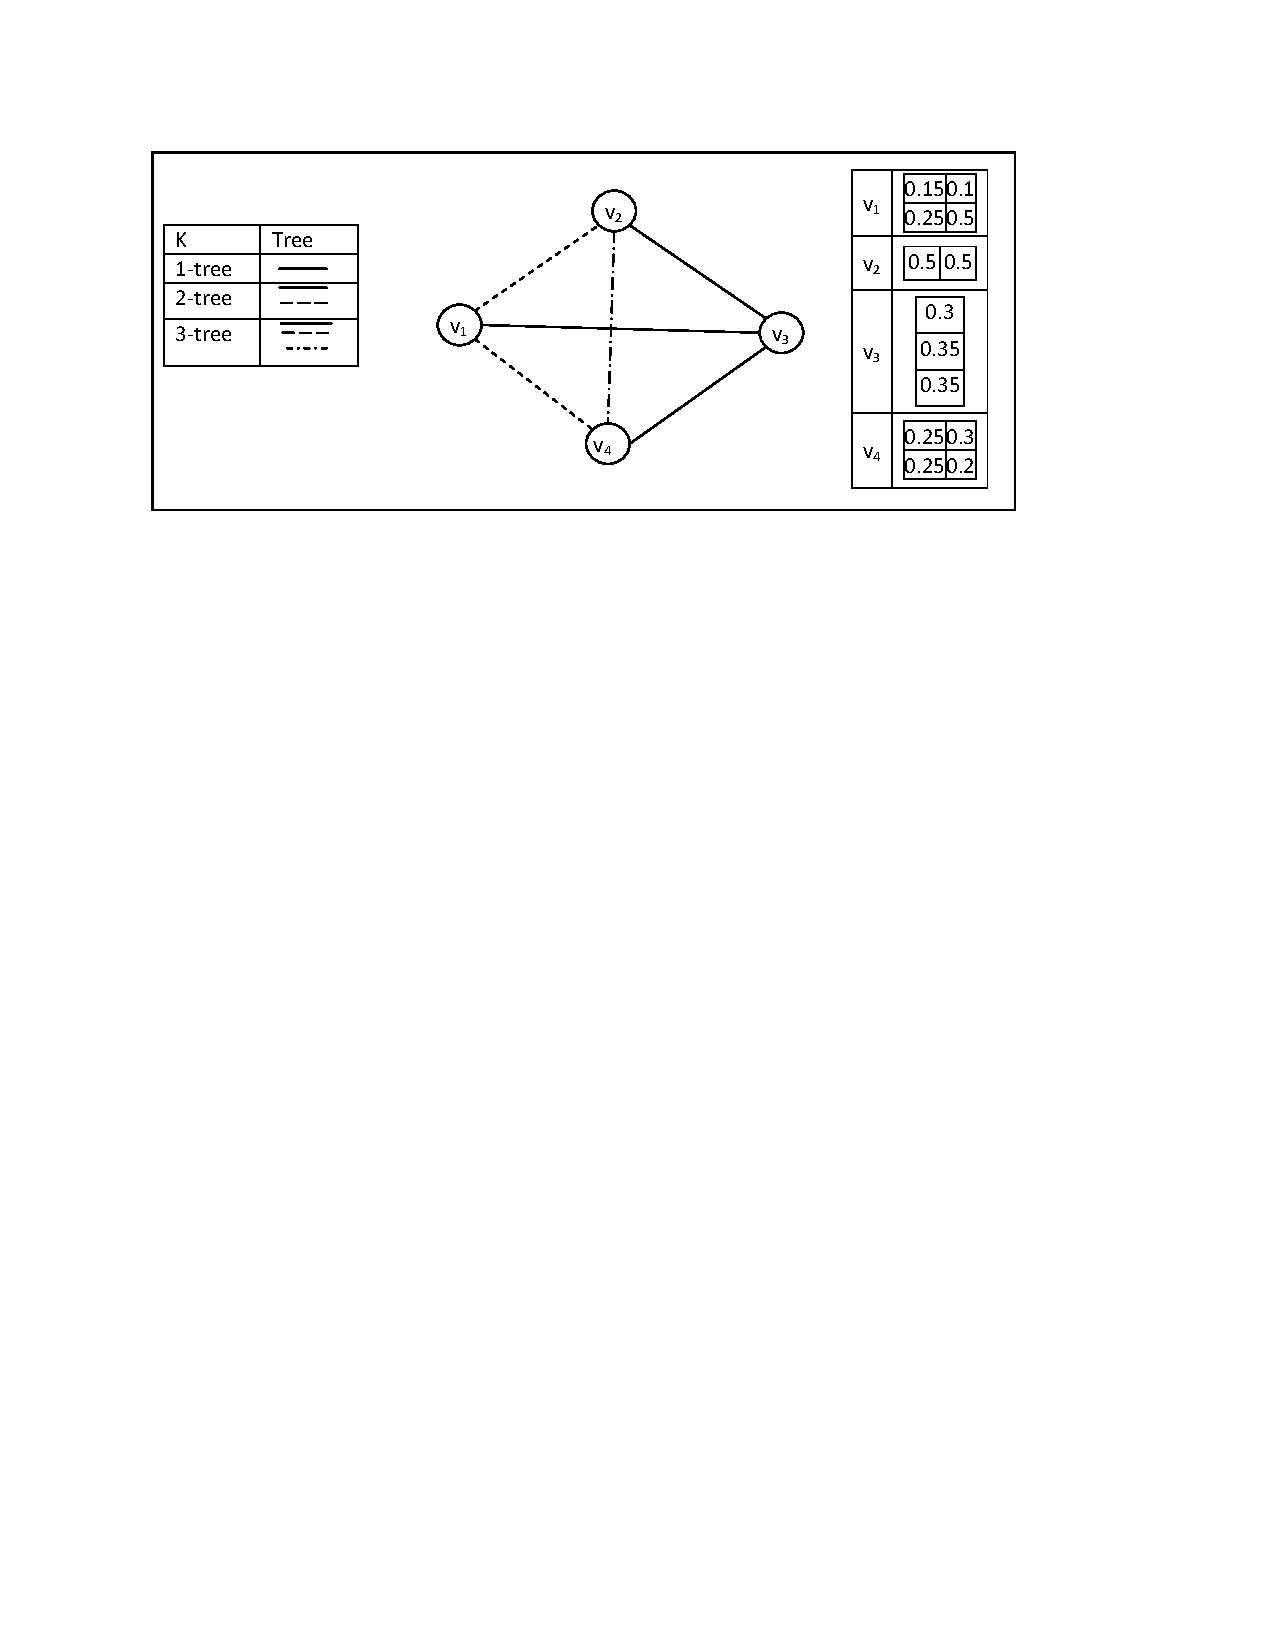
\includegraphics[width=6 in, height=2.5 in]{First_Example.pdf}
 \caption{A partial \(3\)-tree with \(4\) nodes.
}
\end{figure}
 
\begin{exmp}
\normalfont
Fig. 1 illustrates a network of $4$ nodes. Locality set of node $v_1,v_2,v_3$ and $v_4$ has $4,2,3$ and $4$ regions. We are also considering $v_4$ as a sink node. Transmission range \(R_{tr}=8.5\) unit. By using this transmission range node $v_1$ from any of its probable regions can communicate with all probable regions of node $v_2$ and $v_3$ but not with node $v_4$. Similarly node $v_2$ from all probable regions can communicate with all probable regions of node $v_4$ and node $v_1$ but for node $v_3$ only the region with probability value $0.3$. Node $v_3$ can communicate with node $v_4$ when $v_4$ is located in the regions with probability values $0.25$ and $0.2$. $\blacksquare$
\begin{comment}So the probability associated with edges $(v_1,v_2),(v_1,v_3),(v_2,s),(v_2,v_3)$ and $(v_3,s)$ are $1,1,0.85,0.3$ and $0.55$ respectively. $\blacksquare$
\end{comment}
\end{exmp}
 \subsection{Node Connectivity Model}
 %If $Reach(r_{(v,i)},r_{(v',i)})$
If one or more regions in the locality set of node $x\in V$ is within the transmission radius $R_{tr}(y)$ of one or more regions in the locality set of node $y\in V$ and vice-versa then node $x$ is reachable from node $y$.


A network state, $S$ arises when each node is assigned to a specific region from it's locality set. A connected state, $S_{conn}$ is a network state where each node can communicate with others.
\subsection{Problem Statement}
Now we formally define the problem.
\begin{defi}[The $Conn(G,\textbf{R})$ Problem]
\normalfont
Let $G$ is a UWSN where each node $v\in V$ can be located into a set of regions  $R_v=\{r_{(v,1)},r_{(v,2)},....\}$  with probability $p(r_{(v,i})$ where $i=1,2,...$. Also $R_{tr}(v)$ is the transmission radius for node $v\in V$. we would like to find the probability $Conn(G,\textbf{R})$ that each node is connected. $\blacksquare$
\end{defi}

An exhaustive approach to compute $Conn(G,\textbf{R})$ can be 
\begin{itemize}[noitemsep,nolistsep]
\item compute $Reach(r_{(x,i)},r_{(y,j)})$ for every pair of region $r_{(x,i)}, r_{(y,j)}$ where $(x,y)\in V$
\item find all network states $\textbf{S}$ for the given graph $G$.
\item find all connected states $\textbf{S}_{conn}\subset\textbf{S}$ 
\item calculate $Conn(G,\textbf{R})= \sum Pr[S:S\in \textbf{S}_{conn}]$ where $Pr[S]$ can be computed by multiplying all nodes specific regional probability in state $S$.
\end{itemize}
Running time of the exhaustive algorithm can be calculated as follows
\begin{itemize}[noitemsep,nolistsep]
\item let $f(n,\textbf{R})$ is the time to find all network states $\textbf{S}$ for the given graph $G$.
\item let $g(n,\textbf{R})$ the time to find all connected states $S\subset\textbf{S}$
\item in-order to calculate $Conn(G,\textbf{R})$ the upper bound can be $|R_1|\times|R_2|\times..\times|R_n|$. Also let $v$ is the node located maximum number of regions then we can calculate it $|R_1|\times|R_2|\times..\times|R_n|=\mathcal{O}(|R_v|^n)$
\item so the total running time will be $\mathcal{O}(|R_v|^n)$ as $f(n,\textbf{R})$ and $g(n,\textbf{R})$ minor in comparison.
\end{itemize}

 \begin{comment}
If probable location of node \(u\in (V\cup\{s\})\) are \((x_1,y_1),(x_2,y_2),(x_3,y_3),...(x_n,y_n)\) and probable location of node \(v\in (V\cup\{s\})\) are  \((x'_1,y'_1),(x'_2,y'_2),(x'_3,y'_3),...,(x'_n,y'_n)\) and they are connected by an edge \(E\) then the associated probability of the edge can be calculated as follows \(\sum P(x_i,y_i)*P(x'_i,y'_i)\) where the euclidean distance between \((x_i,y_i)\) and \((x'_i,y'_i)\) is less than or equal \(R_s\).

\end{comment}
\section{k-trees}
\label{sec:ktree}
In this section, we will define clique, $k$-tree and perfect elimination sequence which is used in the main algorithm.\\
A clique is a set of vertices that induce a complete subgraph of a graph \(G\). A clique with \(k\) vertices is considered to be a \(k\)-tree.% Treewidth is a parameter which is use to measure how a graph is ``tree like'' or ``close to being a tree''. Treewidth of \(k\) tree is \(k\). 
\begin{defi}
\normalfont
The class of  \(k\)-tree can be  defined recursively as follows: 
\begin{itemize}[noitemsep,nolistsep]
 \item The complete graph on k vertices is a k-tree.
 \item Lets \(G_n\) is a \(k\)-tree  with $n$ vertices where $n\geq k$. Then we can construct a $k$-tree $G_{n+1}$ of $n+1$ vertices by adding a vertex adjacent to exactly $k$ vertices, namely all vertices of a $k$ clique of $G_n$. $\blacksquare$
\end{itemize}

\end{defi}
  A partial \(k\)-tree is any subgraph of a \(k\)-tree . partial \(k\)-trees are rich class of graph. Forest is an example of partial 1-tree. Series-parallel graphs and chordal graphs are subfamily of partial \(2\)-trees. Also Halin graphs, Nested SAT and IO-graphs are subclasses of partial \(3\)-trees.
  
  \begin{comment} Several graph problem that are NP-complete on general graphs have polynomial time algorithms for graphs with treewidth bounded by a constant. Any polynomial time algorithm for graphs of bounded treewidth is a polynomial time algorithm for partial \(k\)-tees.So partial \(k\)-trees are useful as they might be seen as a tool to gain more insight in graphs of bounded treewidth.
  \end{comment} 
  \begin{exmp}
  \normalfont
  Fig. 1 depict a partial $2$-tree. The complete graph of $2$ vertices namely $v_1$ and $v_2$ is a $2$-tree. Then we added vertex $V_3$ which is adjacent to both $v_1$ and $v_2$ is a $2$-tree of $3$ vertices. Finally a vertices $s$ is added to the clique $v_1v_2$ to form the $2$-tree with $4$ vertices.$\blacksquare$
  \end{exmp}
\subsection{Perfect Elimination Sequence}
A perfect elimination sequence (PES) in a graph is an ordering of the vertices of the graph such that, for each vertex $v$, $v$ and the neighbors of $v$ that occur after $v$ in the order form a clique. In-order to find PES we need simplicial vertex.
\begin{defi}[Simplicial Vertex]
\normalfont
A simplicial vertex of a graph $G$ is a vertex $v$ such that the neighbours of $v$ form a clique in $G$. Clearly, if $G$ has a PES, then the last vertex in it is simplicial in G.$\blacksquare$
\end{defi}
\begin{comment}
\begin{defi}[Chordal Graph] 

A graph is chordal if its cycles of four or more vertices has a chord, which is an edge thet is not part of the cycle but connect two vertices of the cycle. $\blacksquare$
\end{defi}

\begin{lemma}
A chordal graph is either complete or has at least two non adjacant simplical vertex\cite{heggernes2006treewidth}.
\end{lemma}
A graph is chordal if and only if it has a PES. There is a corollary that every $k$-tree is a chordal graph \cite{heggernes2006treewidth}. So there is a perfect elimination ordering for every $k$-tree. 
Now in-order to find PES we need to repeat the following step until no simplicial vertices are left: Find a simplicial vertex and remove it from the graph.
If the graph is chordal, there will be a simplicial vertex at each step, by the
above lemma. Therefore, if the remaining graph is not empty at the end of
this process, then we can conclude that the input graph is not chordal. If no
vertices remain at the end of the process, then the order in which the vertices
are removed is called a perfect elimination order.
\end{comment}
\begin{exmp}
\normalfont
In fig. 1 we show that there are two simplicial vertices, $v_1$ and $s$. But $s$ is our sink node so we are not eliminating $s$. So After elimination of $v_1$, we will be able to eliminate either $v_2$ or $v_3$. So the PES will be either $v_1,v_2$ or $v_1,v_3$.$\blacksquare$
\end{exmp}
\section{Main Algorithm}
\label{subsec:mainAlg}
In this section we present an algorithm to compute the exact solution for $Conn(G,\textbf{R})$ problem. More specially, the algorithm  takes as input a UWSN network $G$ where each node has a probabilistic locality set, a PES and compute Prob, a solution to the input $Conn(G,\textbf{R})$ instance. The function uses a dynamic programming framework to solve $Conn(G,\textbf{R})$ problem.\\
\begin{figure}[h]
\centering
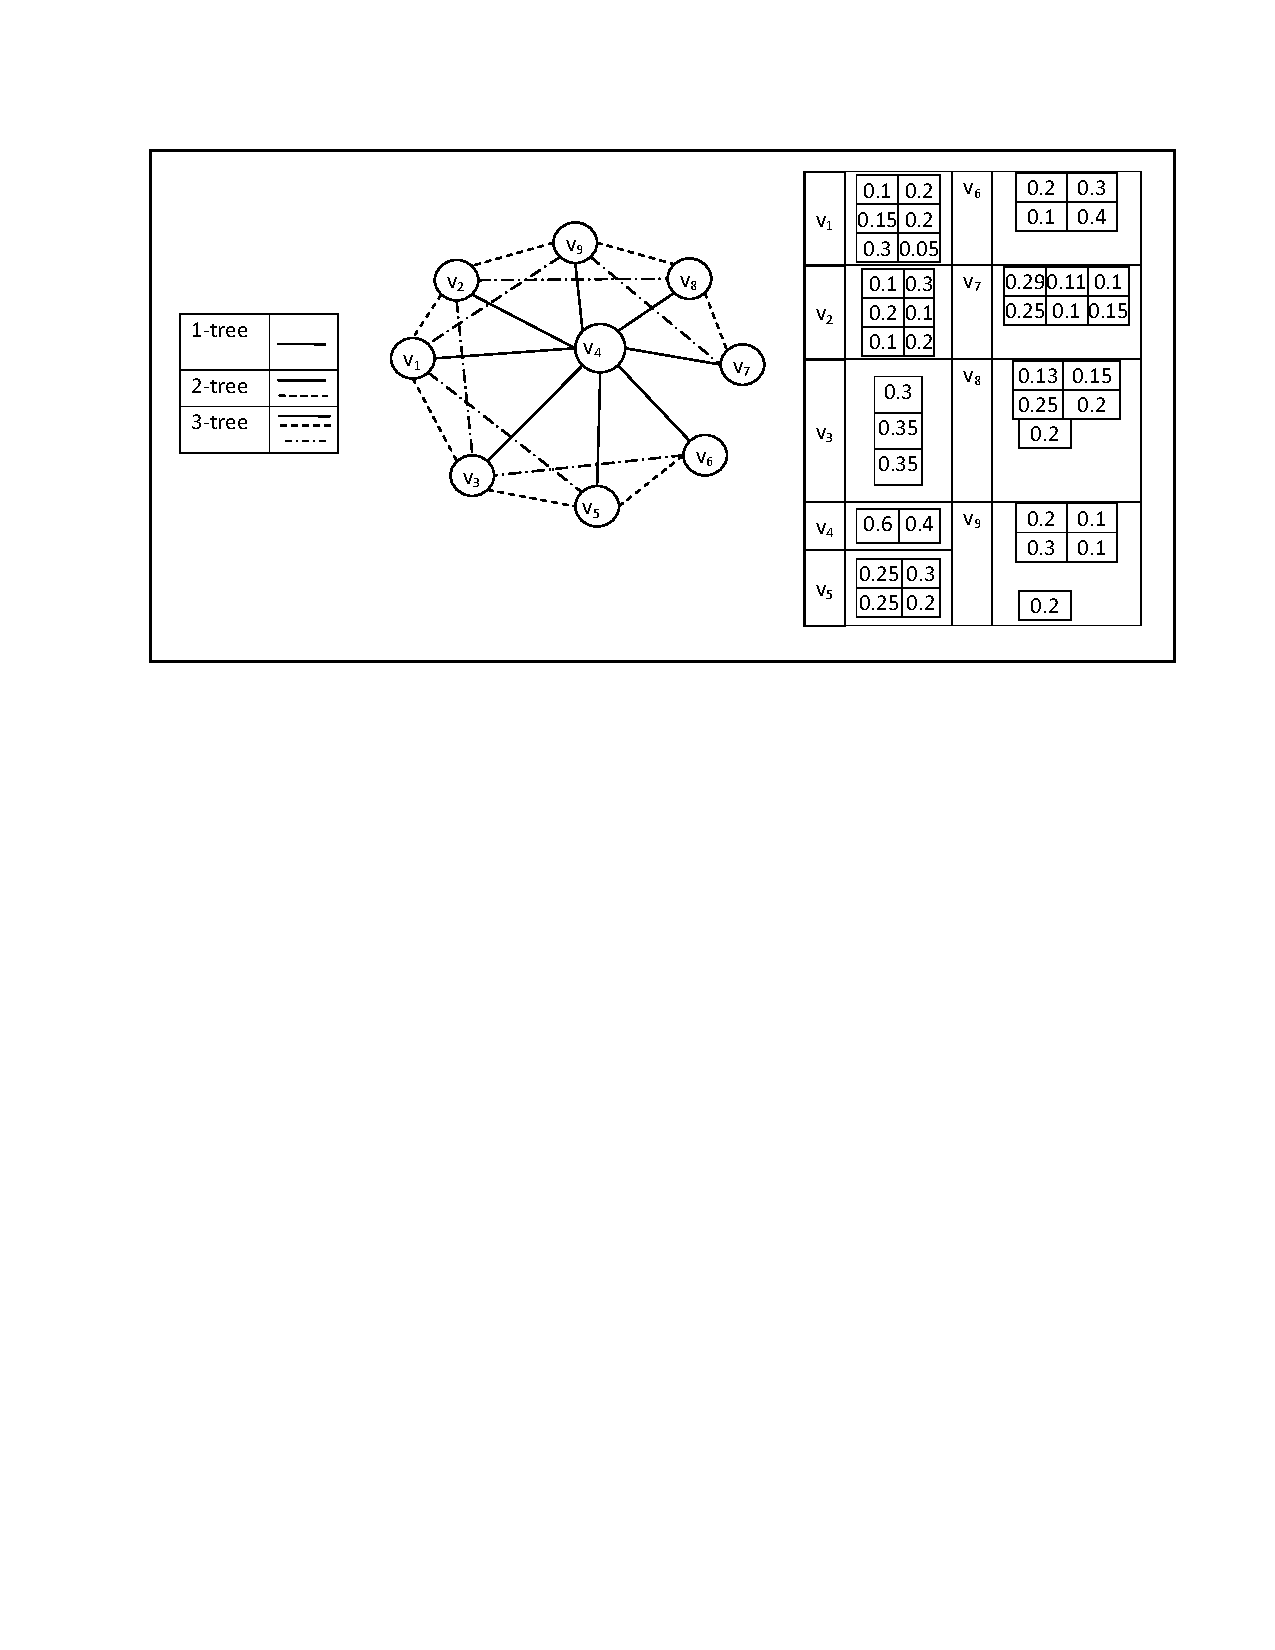
\includegraphics[width=5 in, height=2.5 in]{Example1.pdf}
 \caption{ A UWSN modelled by a $3$-tree.
 \label{fig:3t}
}
\end{figure}
\subsection{Key Data-structures}
\label{subsec:kds}
Each clique associated with a table. Each row in the table defines key-value mapping.
\begin{itemize}[noitemsep,nolistsep]
\item A key is a set of sets namely partition(s) of nodes along with corresponding regions in that particular clique. 
\item A value is a probability which is the multiplication of regional probability of nodes for the clique.
\end{itemize}

\begin{exmp}
\normalfont
Fig. \ref{fig:3t} illustrates a graph $G$ which is a $3$-tree with $9$ nodes and their corresponding probabilistic locality set. There are $19$ triangles so there are $19$ cliques associated with this $3$-tree. For each clique the algorithm maintain a table. For every table there are some rows as key-value mapping. For example the clique $<v_1,v_2,v_3>$  can be partitioned $5$ different ways including $\{v_1,v_2,v_3\}, \{v_1,v_2\}\{v_3\}, \{v_1,v_3\}\{v_2\},\{v_1\}\{v_2,v_3\}$ and $\{v_1\}\{v_2\}\{v_3\} $. For each partition there are  $6\times6\times4=144$ rows as key-value mappings because the locality set of node $v_1,v_2$ and $v_3$ are $6,6$ and $4$ respectively. One of the row is ${\{v_1,v_2,v_3\}}^{(1,1,1)} 0.004$ where $v_1,v_2$ and $v_3$ are in same partition with region $1, 1$ and $1$ respectively and the probability $0.004$ is multiplication of corresponding regional probabilities.$\blacksquare$
\end{exmp}
When the algorithm starts elimination node by the order of $PES$ there will be table merging and details is presented in section \ref{sub:Ald}.
\subsection{Algorithms Description}
\label{sub:Ald}
We now explain the main steps of function main, merge and merge partitions.
\begin{algorithm} [h]
\Indm
\KwIn{ a UWSN $G=(V,E)$ is a partial $k$-tree where each node, $v\in V$  can be located into a set of regions $R_v=\{r_{(v,1)},r_{(v,2)}...\}$ with probability,    
  $\{p(r_{(v,1)}),p(r_{(v,2)})...\}$ and $(x,y)\in E$ if $x\in V$ can be located one of it's locality set and $y\in V$ can be located one of it's locality set, so that they reach each other. $PES$ is a perfect elimination sequence $(v_1,v_2,...,v_{n-k})$ of $G$.}
\KwOut{ Prob, a solution to the input instance.}
\textbf {Notation:} $Temp$ is a map from keys to probabilities.\\
%\noline
\Indp
\nl \textbf{Initialize } every clique by  a table.\\
\nl\For{$i=1,2,...,n-k$}
{
 \nl node $v_i$ is associated with $k$-cliques, $K_{(v_i,1)},K_{(v_i,2)},..,K_{(v_i,k)}$ \\
 //$T_{(v_i,1)},T_{(v_i,2)},..,T_{(v_i,k)}$ are the tables associated with cliques $K_{(v_i,1)},K_{(v_i,2)},..,K_{(v_i,k)}$ respectively \\
\nl $ Temp=T_{(v_i,1)}$  \\
 \nl \For{$j=2,3..,k$}
 {
  \nl $Temp=merge(Temp,T_{(v_i,j)})$\\
 }
 // clique $K_{(v_i,base)}$ is the base clique and table $T_{(v_i,base)}$ is the base table of node $v_i$
  \nl $Temp=merge(Temp,T_{(v_i,base)})$\\
\nl  remove node $v_i$ from $Temp$ and assign the result to $T_{(v_i,base)}$
}

\nl \Return{Prob=$\sum$(All probability for single partition in the remaining table)}
\caption{Function Main$(G$, $\textbf{R}$, $p(r_{(v,i)})$, $PES )$}
\end{algorithm}

\subsubsection{Function Main}
%%Need to writedown main task of this function
Main function eliminates every node according to the PES by merging all cliques associated with that node and updating the result to base clique. The last remaining clique associates with the sink node. Finally  main function calculates the connectivity from the last clique by adding probabilities for those row which is associate with single partition.

In more details, 
\begin{itemize}[noitemsep,nolistsep]
\item   Step $1:$ initialize each clique by a table describe in subsection \ref{subsec:kds}.
\item Step $2:$ processes each node $v_i$ in PES. Every processing node, $v_i$ is associated with $k$ cliques.
\item Step $3:$ finds all those cliques,
 $K_{(v_i,1)},K_{(v_i,2)},..,K_{(v_i,k)}$. 
 \item Step $4:$ assign table $Temp$ with table  $T_{(v_i,1)}$ associated with clique  $K_{(v_i,1)}$.
 \item Steps $5$-$6:$ iteratively merge all associated tables of node $v_i$ and assign the result to table $Temp$ by using $merge$ function. \item Step $7:$ merge $Temp$ table with base table of node $v_i$ $T_{(v_i,base)}$ by using $merge$ function and assign the result to $Temp$. 
 \item Step $8:$ remove the vertex $v_i$ and it's locality set from $Temp$ and assign the result to $T_{(v_i,base)}$.
 \item Step $9:$ calculate and return connectivity for the network.
 \end{itemize}
\begin{exmp}
\normalfont
 One of the PES of the $3$-tree depict in fig. \ref{fig:3t} is $<v_1,v_6,v_5,v_7,v_8, v_9>$. In-order to eliminate $v_1$, the algorithm  merge three cliques $<v_1,v_3,v_4>$, $<v_1,v_2,v_3>$ and $<v_1,v_2,v_4>$ to $<v_1,v_2,v_3,v_4>$. Next step the algorithm find the base clique $<v_2,v_3,v_4>$ and merge with  $<v_1,v_2,v_3,v_4>$. Finally it deletes $v_1$  from merged clique and update the result to $<v_2,v_3,v_4> \blacksquare$
\end{exmp}
\begin{table}[!htb]
    %\caption{Global caption}
    \begin{minipage}{.3\linewidth}
      %\caption{$T_1(v_1,v_2,v_3)$}
      \centering
     \begin{tabular}{cc}
\multicolumn{2}{c}{$T_1(v_1,v_2,v_3)$}                           \\ \hline
\multicolumn{1}{|c}{.} & \multicolumn{1}{|c|}{.} \\ \hline
\multicolumn{1}{|l}{$\{v_1,v_2\}^{(1,1)} \{v_3\}^{(2)}$} & \multicolumn{1}{|l|}{$0.002$} \\ \hline
                             \multicolumn{1}{|c}{.} & \multicolumn{1}{|c|}{.} \\ \hline               
                   \multicolumn{1}{|c}{.} & \multicolumn{1}{|c|}{.} \\ \hline
                   \multicolumn{1}{|c}{.} & \multicolumn{1}{|c|}{.} \\ \hline        
\end{tabular}
    \end{minipage}%
    \begin{minipage}{.05\linewidth}
      %  \centering
     % \caption{•}
        \begin{tabular}{c}
     $ \times$\\
        \end{tabular}
    \end{minipage}%
     \begin{minipage}{.3\linewidth}
      %\caption{$T_1(v_1,v_2,v_3)$}
      \centering
     \begin{tabular}{cc}
\multicolumn{2}{c}{$T_2(v_1,v_3,v_4)$}                           \\ \hline
\multicolumn{1}{|c}{.} & \multicolumn{1}{|c|}{.} \\ \hline
\multicolumn{1}{|l}{$\{v_1\}^{(1)}\{v_3,v_4\}^{(2,1)}$} & \multicolumn{1}{|l|}{$0.008$} \\ \hline
                   \multicolumn{1}{|c}{.} & \multicolumn{1}{|c|}{.} \\ \hline               
                   \multicolumn{1}{|c}{.} & \multicolumn{1}{|c|}{.} \\ \hline
                   \multicolumn{1}{|c}{.} & \multicolumn{1}{|c|}{.} \\ \hline        
\end{tabular}
    \end{minipage}%
      \begin{minipage}{.06\linewidth}
      %  \centering
     % \caption{•}
        \begin{tabular}{c}
     $ \Rightarrow$\\
        \end{tabular}
    \end{minipage}%
     \begin{minipage}{.3\linewidth}
      %\caption{$T_1(v_1,v_2,v_3)$}
      \centering
     \begin{tabular}{cc}
\multicolumn{2}{c}{$Temp(v_1,v_2,v_3,v_4)$}                           \\ \hline
\multicolumn{1}{|c}{.} & \multicolumn{1}{|c|}{.} \\ \hline
  \multicolumn{1}{|l}{$\{v_1,v_2\}^{(1,1)}\{v_3,v_4\}^{(2,1)}$} & \multicolumn{1}{|l|}{$0.0008$} \\ \hline         
                   \multicolumn{1}{|c}{.} & \multicolumn{1}{|c|}{.} \\ \hline                 
                   \multicolumn{1}{|c}{.} & \multicolumn{1}{|c|}{.} \\ \hline
                   \multicolumn{1}{|c}{.} & \multicolumn{1}{|c|}{.} \\ \hline        
\end{tabular}
    \end{minipage}\\
    \begin{minipage}{1.0\linewidth}
       \centering
     % \caption{•}
        \begin{tabular}{c}
Figure 3 a). Merging two table into $Temp$
        \end{tabular}
    \end{minipage}\\
     \begin{minipage}{.4\linewidth}
      %\caption{$T_1(v_1,v_2,v_3)$}
      \centering
     \begin{tabular}{cc}
\multicolumn{2}{c}{$Temp(v_1,v_2,v_3,v_4)$}                           \\ \hline
\multicolumn{1}{|c}{.} & \multicolumn{1}{|c|}{.} \\ \hline
  \multicolumn{1}{|l}{$\{v_1,v_2\}^{(1,1)}\{v_3,v_4\}^{(2,1)}$} & \multicolumn{1}{|l|}{$0.0008$} \\ \hline         
                   \multicolumn{1}{|c}{.} & \multicolumn{1}{|c|}{.} \\ \hline                 
                   \multicolumn{1}{|c}{.} & \multicolumn{1}{|c|}{.} \\ \hline
                   \multicolumn{1}{|c}{.} & \multicolumn{1}{|c|}{.} \\ \hline        
\end{tabular}
    \end{minipage}%
     \begin{minipage}{.06\linewidth}
      %  \centering
     % \caption{•}
        \begin{tabular}{c}
     $ \Rightarrow$\\
        \end{tabular}
    \end{minipage}%
    \begin{minipage}{.3\linewidth}
      %\caption{$T_1(v_1,v_2,v_3)$}
      \centering
     \begin{tabular}{cc}
\multicolumn{2}{c}{$Temp(v_2,v_3,v_4)$}                           \\ \hline
\multicolumn{1}{|c}{.} & \multicolumn{1}{|c|}{.} \\ \hline
  \multicolumn{1}{|l}{$\{v_2\}^{(1)}\{v_3,v_4\}^{(2,1)}$} & \multicolumn{1}{|l|}{$0.0008$} \\ \hline         
                   \multicolumn{1}{|c}{.} & \multicolumn{1}{|c|}{.} \\ \hline                 
                   \multicolumn{1}{|c}{.} & \multicolumn{1}{|c|}{.} \\ \hline
                   \multicolumn{1}{|c}{.} & \multicolumn{1}{|c|}{.} \\ \hline        
\end{tabular}
    \end{minipage}\\
      \begin{minipage}{1.0\linewidth}
       \centering
     % \caption{•}
        \begin{tabular}{c}
Figure 3 b). Deleting node $v_1$ from $Temp$
        \end{tabular}
    \end{minipage}\\
\end{table}
\subsubsection{Function merge}
The primary task of merge function is to merge two table $T_1, T_2$, update keys and values of the newly created table $T$ and return the table $T$.

In more details, 
\begin{itemize}[noitemsep,nolistsep]
\item Step $1:$ finds the common vertices between two tables  and assign the common nodes probability $1$.
\item Step $2:$  check if whether or not the common vertex set $C$ is empty. If it is empty then the algorithm returns otherwise go to next step. 
\item Steps $3$-$5:$  performs the row-wise merging by using function $mpar$ and create another row.
\item  Steps $6$-$7:$ updates the locality set for every vertex $v$ of newly created row. 
\item Steps $8$-$9:$ calculates the regional probability of common nodes. 
\item Step $10:$ updates the newly created row probability by multiplying row-wise probability and dividing by the sum of common nodes regional probabilities. 
\item Step $11:$ insert the row into table $T$ and 
\item Step $12:$ return table $T$.
\end{itemize}
\begin{exmp}
\normalfont
Fig 3 a). illustrates merging row  $\{v_1,v_2\}^{\{1,1\}}\{v_3\}^{\{2\}}$ $0.002$ of table $T_1$ with row $\{v_1\}^{\{1\}}\{v_3,v_4\}^{\{2,1\}}$ $0.008$ of table $T_2$ which is fundamental operation for merging two tables. The function merge uses $pMerge$ function which takes two partitions $\{v_1,v_2\}\{v_3\}$ and $\{v_1\}\{v_3,v_4\}$ and returned $\{v_1,v_2\}\{v_3,v_4\}$ because $\{v_1,v_2\}\cup \{v_1\}=\{v_1,v_2\}$ and $\{v_3\}\cup \{v_3,v_4\}=\{v_3,v_4\}$. The merge function updates the locality set of each node of the merged partition $\{v_1,v_2\}^{\{1,1\}}\{v_3,v_4\}^{\{2,1\}}$ from the locality set of nodes in merging partitions. There are two common nodes $v_1$ and $v_3$ located in region $1$ and $2$ respectively with probability $0.1$ and $0.2$ respectively in the merging partitions. It update the probability of newly created partition $0.0008$ by multiplying row-wise probabilities $0.002\times 0.008$ and dividing the probability by product of the common nodes corresponding regional probabilities $0.1\times 0.2$.

Fig 3 b). shows the deletion of node $v_1$ from $Temp$. The function main simply look for the node and remove it and it's locality set from key.$\blacksquare$
\end{exmp}
\begin{algorithm}[H]
\Indm  
\KwIn{ Two tables $T_1$ and $T_2$ that share at least one common vertex}
\KwOut{A  table $T$}

\textbf{Notation} $C$ is a set of vertices and $Obj$ is a row of table $T$ and $Prob\_C$ is a double variable\\
\Indp
\nl \textbf{set} $C=$ the set of common vertices between $T_1$ and $T_2$ , set $Prob\_C=1$\\
 \nl \If{$C\neq \emptyset$}{
 \nl \ForEach{row $r$ in $T_1$}
 {
 \nl \ForEach{row $s$ in $T_2$}
 {
  \nl  $Obj.par=$pMerge($r.par$,$s.par$)\\
   \nl \ForEach{vertex $v_i$ in $Obj.par$ where $i=1,2,..,k+1$}
    {
   \nl $Obj.loc[v_i]=r.loc[v_i]||s.loc[v_i]$\\
    }
    
   \nl \ForEach{vertex  $v\in C$}
    {
   \nl $Prob\_C=Prob\_C*s.loc[v]$
    }
\nl $ Obj<Obj.par:Obj.loc>=\frac{Prob[r]\times Prob[s]}{Prob\_C}$\\
\nl Insert $Obj$ in $T$ as a row.\\
}
  }
  }
\nl \Return {Table T}

 \caption{Function merge($T_1,T_2$)}
\end{algorithm}

\subsubsection{Function Merge Partitions }
 The merging partitions is mainly done using the union operation by mapr function. The mpar function takes as input two partitions $P_1$, $P_2$ and merge them into one partition $P$.

In more details,  
\begin{itemize}[noitemsep,nolistsep]
\item Steps $1$-$2:$ adds all the sets of $P_2$ to $P_1$.
\item Steps $3$-$4:$ selects two sets $s^*$ and $t^*$ from partition $P_1$ 
\item Step $5$: checks whether or not they are disjoint . If they are  not disjoint then it will go to step 6 otherwise it will return to step 4.
\item Step $6:$ delete $s^*$ from $P_1$.
\item Step $7:$ computes the union of $s^*$ and $t^*$ and insert it at the beginning of partition $P_1$.
\item Step $8:$ delete $t^*$ from $P_1$.
\item Steps $9$-$10:$ set the iterator to the beginning of $P_1$ and return to step 5.
\item Step $11:$ assign $P_1$ to $P$ and finally the algorithm return $P$.
\end{itemize}


\begin{algorithm}[H]
\KwIn{Two partitions $P_1$ and $P_2$}
\KwOut{A partition $P$}
\textbf{Notation:} $s$ and $t$ are two set iterators and their corresponding set are indicated by $s^*$ and $t^*$.\\ 
\nl \ForEach{ set $s^*$ in $P_2$}
{
\nl $P_1.push\_back(s^*)$
}
\nl \For{ $(s=P_1.begin()$; $s \neq P_1.end()$;  $++s)$}
{
\nl \For{ $(t=s.next()$; $t \neq P_1.end()$; $++t)$}
{
 \nl \If{$s^*\cap t^* \neq \emptyset$}
  {
\nl   $P_1.delete(s^*)$\\
\nl	$  P_1.push\_front(s^*\cup t^*$)\\
  \nl $P_1.delete(t^*)$\\
  \nl $s=P_1.begin()$\\
   \nl$break$\\
  }
}
}
\nl set $P=P_1$\\
\Return{P}
\caption{function pMerge($P_1$, $P_2$)}
\end{algorithm}


%COMMENT
\begin{comment}Step 2 initializes every clique by $k$ nodes. In this step $k$ nodes along with their locality set forms partitions. If $k$ nodes are in the same partitions then they will be in the same sub-tree otherwise they will be in different sub-tree. For every set of partition(s) there is a probability which is from corresponding regional probability
 For every edge $(v_1,v_2)\in E$ if the probable regions for node $v_1$ in a certain time instant are $\Re=\{R_1,R_2,...,R_n\}$  with probability $P(R)=\{P(R_1),P(R_2),...,P(R_n)\}$ and if the probable regions for node $v_2$ are $R'=\{R'_1,R'_2,...,R'_m\}$   with probability $P(R')=\{P(R'_1),P(R'_2),...,P(R'_m)\}$. We are considering that each region is rectangular and we are placing the sensor node at the point where diagonals of the rectangle intersect. In-order to make implementation simpler, we present each node and their set of regions by integer number. Every row in the table consists of one or more partition followed by region number and edge probability is the last entry in the row. After getting the euclidean distance between two sensors position of two regions of two different nodes, we compare it with transmission range $R_{tr}$. If the euclidean distance is less than equal to $R_{tr}$ then we add two rows in the table. First row consists of a single partition of nodes in-order to show they are in same tree, followed by their regions number followed by probability value which is the multiplication of  the probability associated with those two regions. Second row we will show these two  nodes will be in different partition in-order to show that the node are in different tree, for corresponding regions with probability value $0$. If the euclidean distance is greater than the transmission range then we place two node in two different partition followed by their corresponding region followed by a probability which is multiplication of the corresponding regions probability value. For example of edge $(v_1,v_2)\in E$ if the euclidean distance between region $\mathfrak{R_i}$ sensor position and $\mathfrak{R'_j}$ sensor position is less than $R_{tr}$ then two entry will be $\{v_1,v_2\} $ $\mathfrak{R_i}$  $ \mathfrak{R'_j}$  $ P(\mathfrak{R_i}) * P(\mathfrak{R'_j})$ and $\{v_1\} \{v_2\} $ $\mathfrak{R_i}$ $ \mathfrak{R'_j}$  $ 0$ and if the distance is greater than $R_{tr}$ then there will be only one entry $\{v_1\} \{v_2\} $ $\mathfrak{R_i}$  $ \mathfrak{R'_j}$  $ P(\mathfrak{R_i}) * P(\mathfrak{R'_j})$ in the table where $ i=1,2,3,...,n $ and $j=1,2,3,...,m$.

\begin{figure}
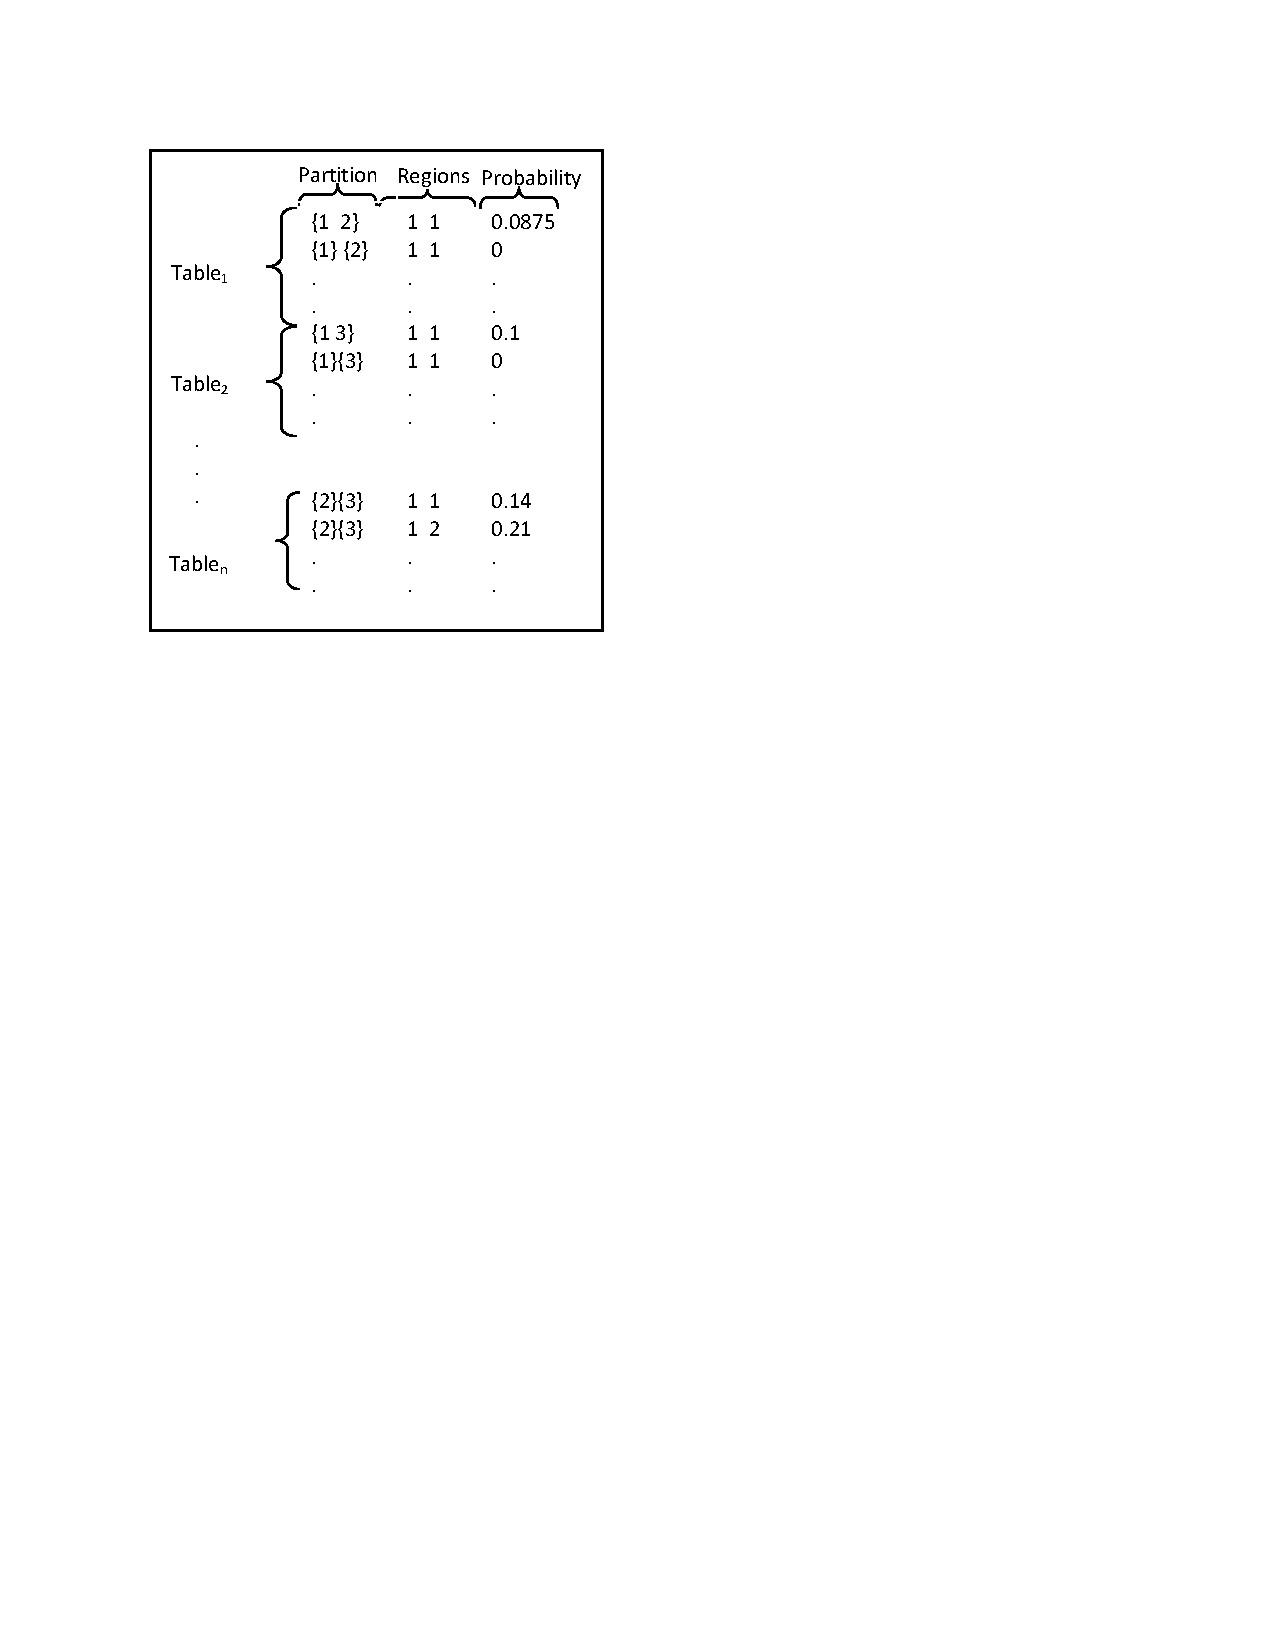
\includegraphics[width=3 in, height=2.5 in]{Table.pdf}
 \caption{ a typical database.
}
\end{figure}
\end{comment}




%COMMENT
\begin{comment}  Then we will put two entry in edge table $\{(x_i,y_i),(x'_j,y'_j)\}:p(x_i,y_i)*p(x'_j,y'_j)$ and  $\{(x_i,y_i)\} \{(x'_j,y'_j)\}: 0$ otherwise we will put  $\{(x_i,y_i)\} \{(x'_j,y'_j)\}:p(x_i,y_i)*p(x'_j,y'_j)$.
Now we will merge edge table to find a table for a clique as follows. Let's there is a entry in the edge table between node $i$ and $j$ is $\{(x_i,y_i),(x'_j,y'_j)\}:p(x_i,y_i)*p(x'_j,y'_j)$. We will be able to merge the above entry to another entry in different edge table if there is a common node location in same position as previous edge table entry. For example if there is another entry in the edge table between node $i$ and $k$ is $\{(x_i,y_i),(x''_k,y''_k)\}:p(x_i,y_i)*p(x''_k,y''_k)$. So after merging the new entry will be $\{(x_i,y_i),(x'_j,y'_j),(x''_k,y''_k)\}:\frac{p(x_i,y_i)*p(x'_j,y'_j)*p(x_i,y_i)*p(x''_k,y''_k)}{p(x_i,y_i)}$. 

\end{comment}
\subsection{Verification Cases}
\label{subsec:vc}
In this subsection we are going to present some cases by using these one can verify the correctness of our algorithm.
\begin{figure}
\label{fig:var}
\begin{minipage}{.9\linewidth}
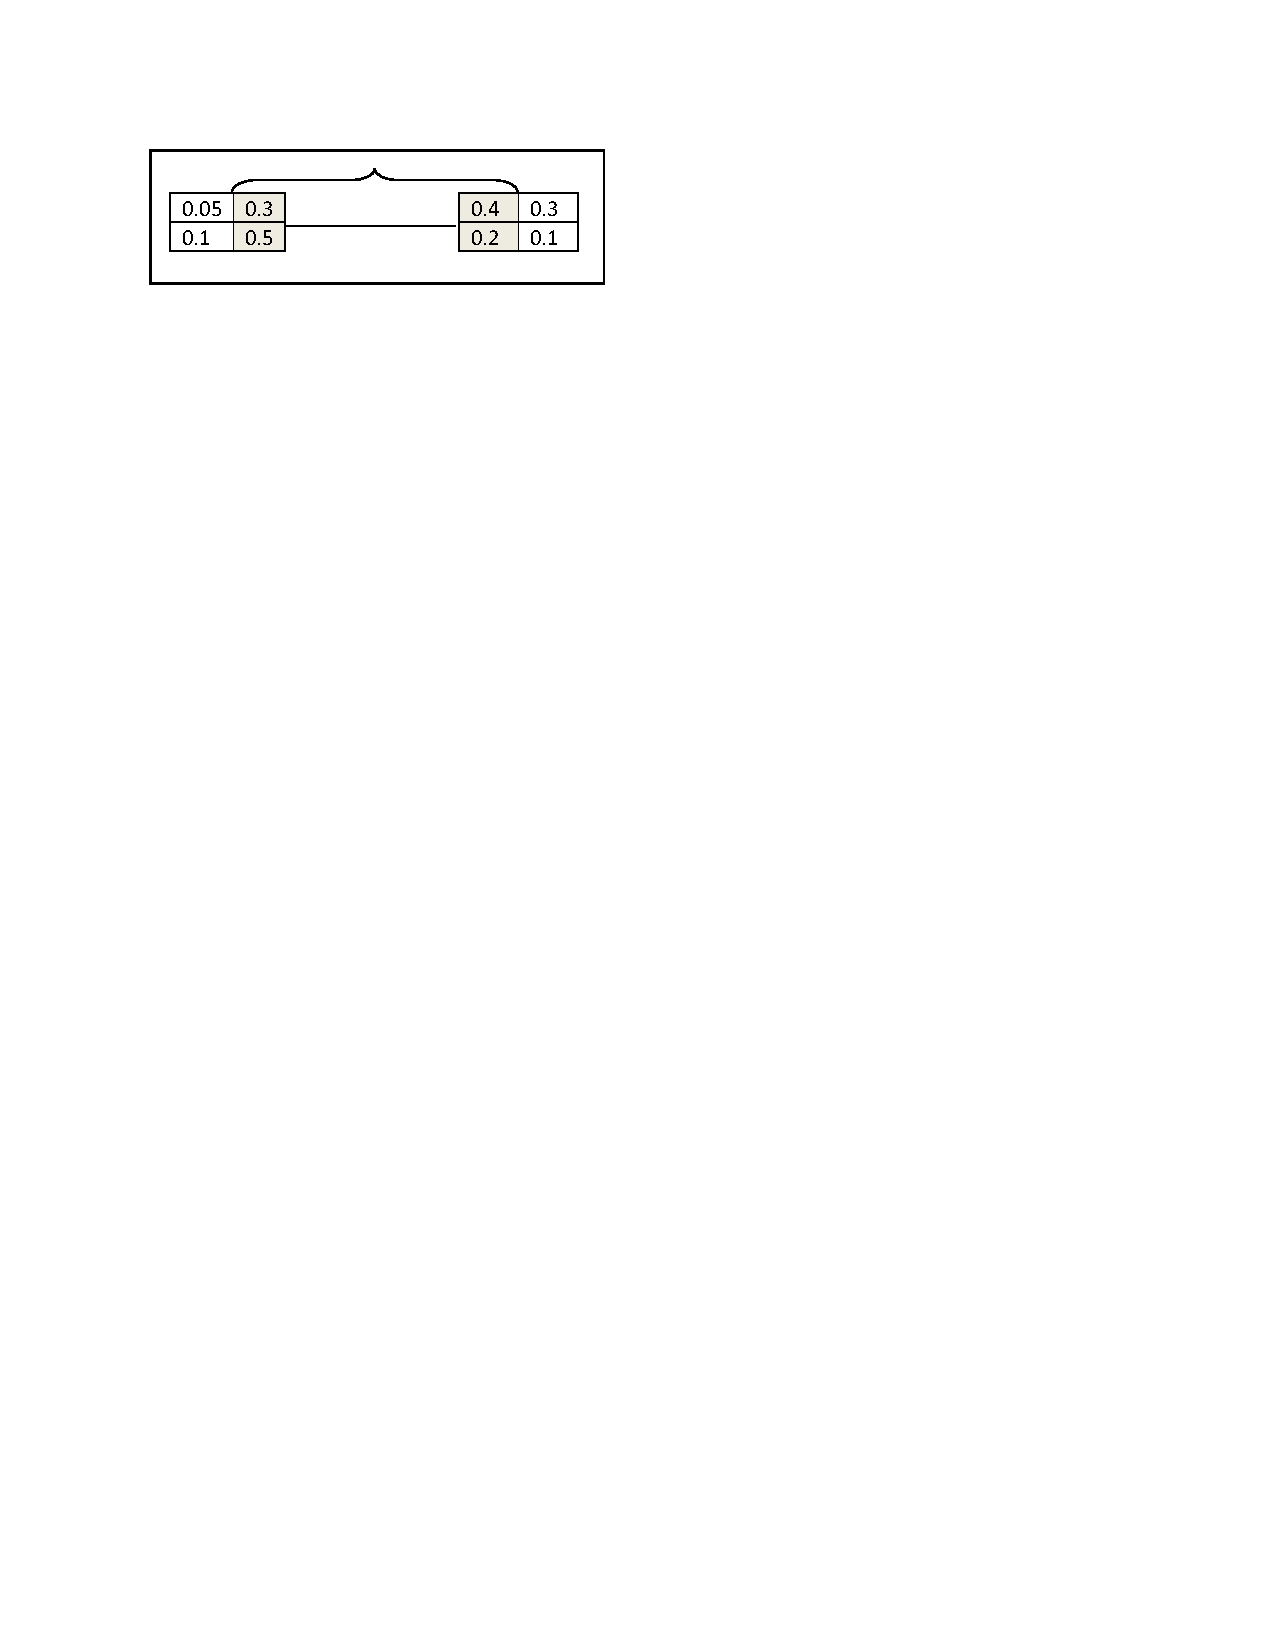
\includegraphics[width=3 in, height=.6 in]{verification.pdf}
\caption{A simple tree with 2 nodes}
\end{minipage}
\end{figure}
\begin{itemize}
\item For a partial $k$-tree, there should be more than one PES. In our algorithm, we tried all elimination sequence and we got same result.
\item The algorithm exhaustively consider all possible configuration to calculate the connectivity. Consider a small example with two nodes illustrates in fig \ref{fig:var} where $v_1$ and $v_2$ has the locality set of four for both nodes. In-order to find connectivity the algorithm consider all possible configuration and there are $16$ possible configurations. But $v_1$ can reach node $v_2$ when $v_1$ is in regions with probability $0.3$ and $0.5$ and $v_2$ is in regions with probability $0.4$ and $0.2$. So the connectivity for this small network is $0.8 \times 0.6=0.48$.

\end{itemize}

\subsection{Correctness}
In this section we prove the correctness of our algorithm. It is an exhaustive algorithm which takes care all possible configuration.
Our algorithm consists of two fundamental operation, partition merge and table merge. First we prove that partition merge and table merge are correct then we prove that our algorithm is correct.\\
 The partition merge perform core operations of the algorithm. The partition merge is correct because it is merging two partitions into one given that they share at least one node. The table merge is correct because of the following reason. The table merge is merging each row of one table with each row of another table by holding the condition that they share atleast one node with same regional position. It is using partition merge in-order to merge two rows which is correct. The main algorithm is elimination a node by merging all clique associated with that node and updating the merged clique with base clique of that node. Each clique is associated with table so cliques are merged by using table merge operation which is correct. That concludes that the algorithm is correct.
\subsection{Running time}
\begin{itemize}[noitemsep]
\item The number of nodes in a table for $k$-tree $=k$.
\item The number of ways $k$ nodes can be partitioned $=2^k$.
\item locality set of a node which is largest in comparison with other nodes $=l_{max}$.
\item The number of ways each partition reappear $=l_{max}^k$.
\item So the length of a table $=l_{max}^k \times 2^k$.
\item In-order to merge two tables total number of operation$=(l_{max}^k \times 2^k)^2$.
\item When we are elimination a node the number of clique associated with a node for $k$-tree$=k$ and there is one base clique associated with every clique. So total number of clique associated with a node $=k+1$.
\item Total number of operation to eliminate one node $=(l_{max}^k \times 2^k)^{k+1}$
\item Total number of node we are eliminating $=N$.
\item So the total cost $=N \times( l_{max}^k \times 2^k)^{k+1}$
\
\end{itemize}

\section{Simulation Results}
In this section we present simulation results that aim to investigate the following aspect 
\begin{itemize}
\item[(a)] complexity of our algorithm increases with increasing the value of $k$ for partial $k$-tree.
\item[(b)] influence of $k$ on accuracy where $k=1,2,3,..$.
\item[(c)] effect of choosing different $k$-trees.
\end{itemize}
 
\begin{table}[!htb]
    %\caption{Global caption}
    \begin{minipage}{.5\linewidth}
    \caption{Running time (RT) with respect to $k$}
      \centering
     \begin{tabular}{|c|c|c|c|}
     \hline
         k& Network I & Network II & Network III \\
     \hline
     1&30& 30& 20 \\\hline
     2&290 &380&380	\\\hline
3 &85000&875000&940000	 \\\hline
 



\end{tabular}
    \end{minipage}
    \begin{minipage}{.5\linewidth}
      \caption{Accuracy with respect to $k$}
      \centering
     \begin{tabular}{|c|c|c|c|}
     \hline
     k& Network I & Network II & Network III \\
     \hline
      1 & 62&32.96& 81.8 \\\hline
2 &71.2 & 36.15& 98.95\\\hline
3 &75& 37.31& 100\\\hline
\end{tabular}
    \end{minipage}\\
   % \caption{Running time(RT) and accuracy increases with respect to $k$}
    
\end{table}


\begin{figure}
\begin{minipage}{.9\linewidth}
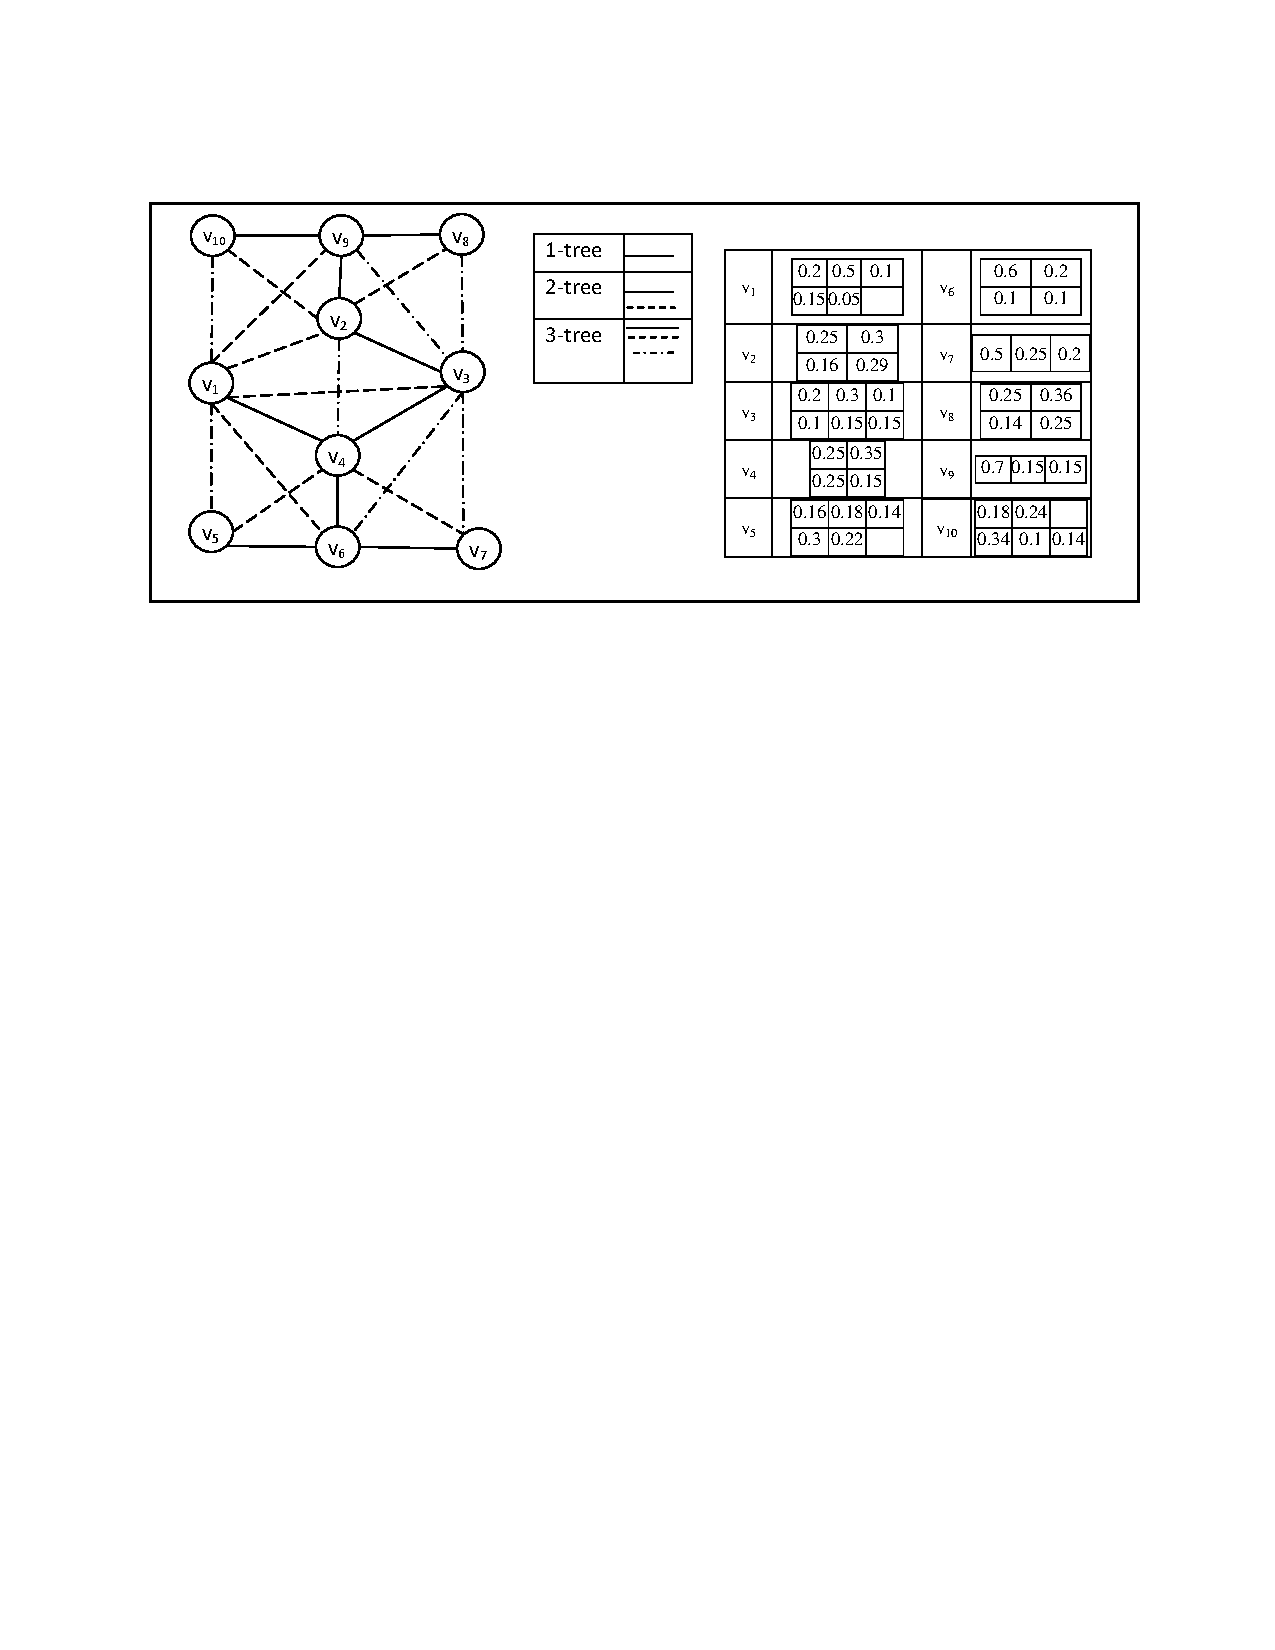
\includegraphics[width=6 in, height=2.8 in]{netI.pdf}
\caption{NetworkI}
\end{minipage}
\begin{minipage}{.9\linewidth}
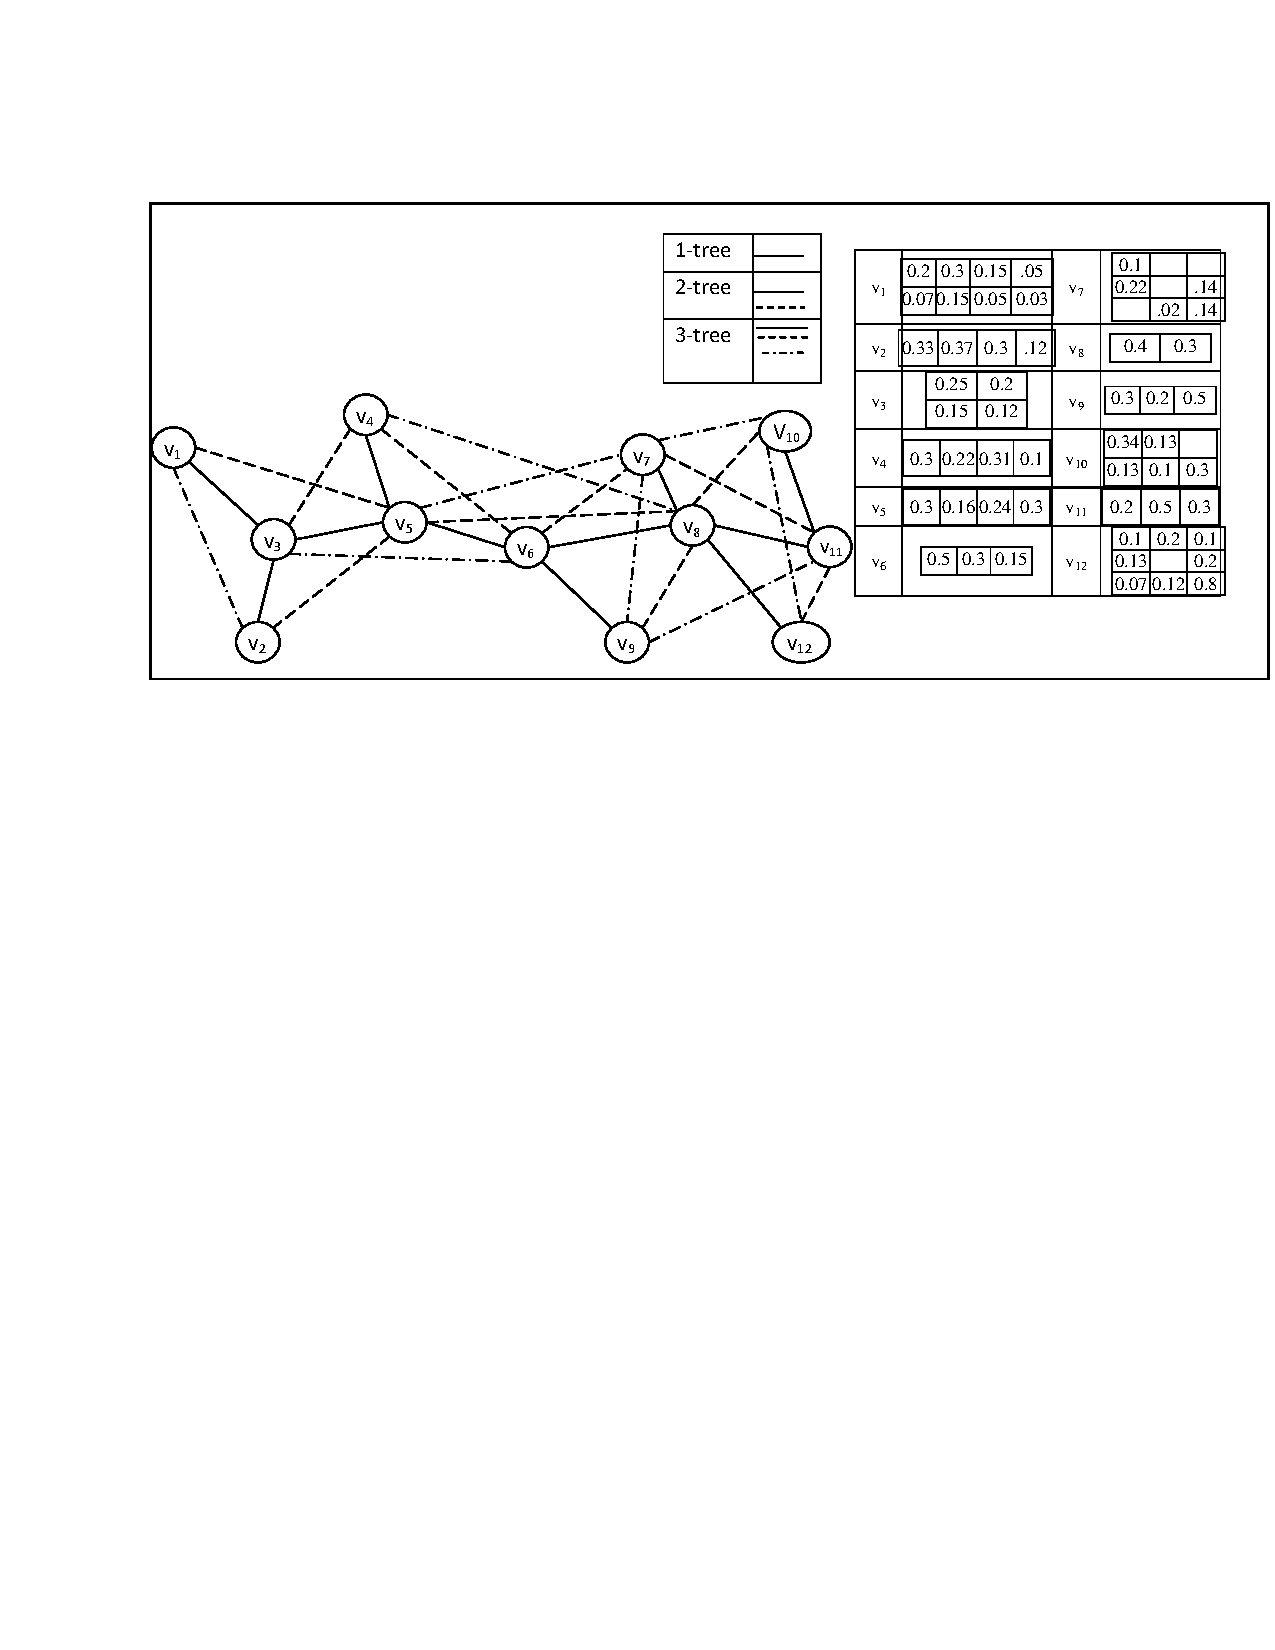
\includegraphics[width=6 in, height=2.7 in]{NetworkII.pdf}
\caption{NetworkII}
\end{minipage}
\begin{minipage}{.9\linewidth}
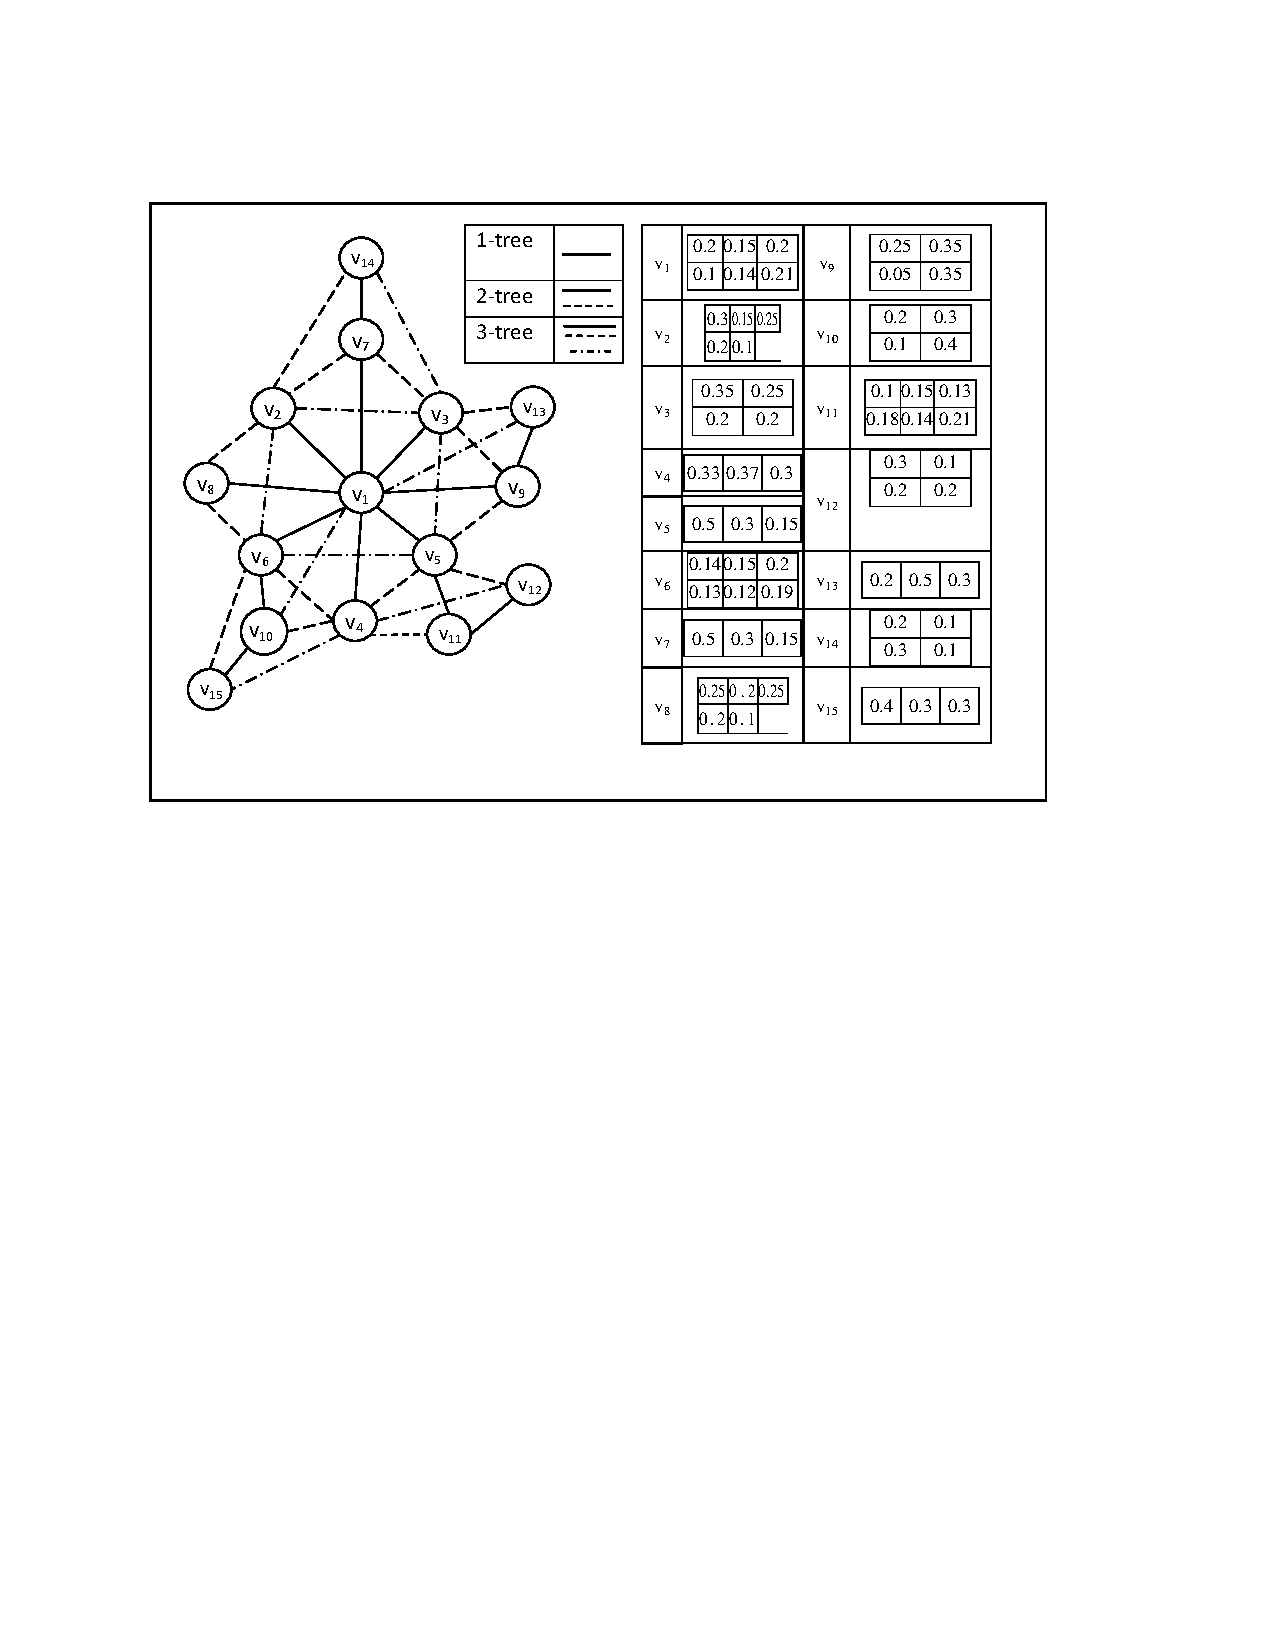
\includegraphics[width=6 in, height=2.6 in]{NetworkIII.pdf}
\caption{NetworkIII}
\end{minipage}

\end{figure}
We used three networks in-order represent running time and accuracy. Network I consists of $7$ nodes with locality set of each node range from $4$ to $8$. Network II consists of $9$ nodes where each node can be located from $3$ to $6$ locations.Network III consists of $12$ nodes with locality set of each node range from $2$ to $8$.
\begin{figure}
\begin{minipage}[]{.5\linewidth}
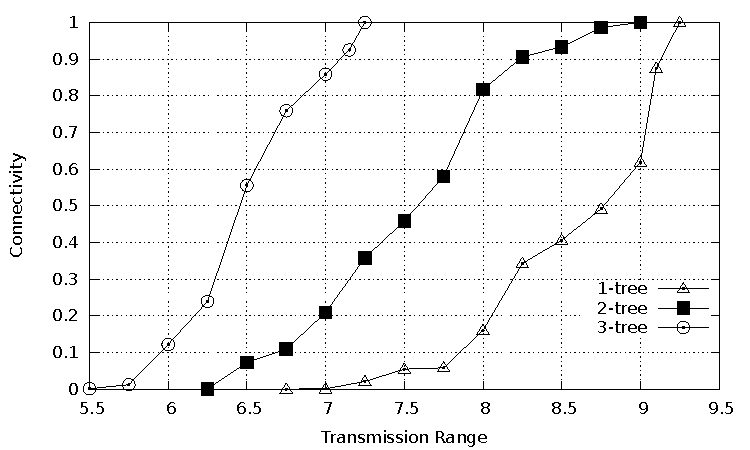
\includegraphics[width=3 in, height=2.5 in]{random.pdf}
 \caption{ Connectivity versus transmission range with  random edge selection.
}
\label{fig:res}
\end{minipage}
\begin{minipage}{.5\linewidth}
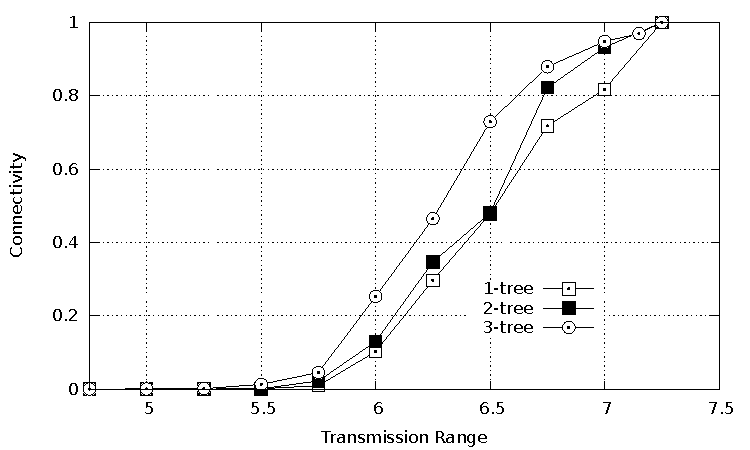
\includegraphics[width=3 in, height=2.5 in]{Greedy.pdf}
 \caption{ Connectivity versus transmission range with greedy edge selection.
}
\label{fig:ges}
 \end{minipage}
\end{figure}
\begin{itemize}
\item[a)] \textbf{$k$ versus running time} table 1 shows three scenarios running time with respect to $k$ of. In every scenario the running time of the algorithm increases with $k$. We also observe that difference between the running time $1$-tree and $2$-tree are $10$ to $15$ times where the running time between $2$-tree and $3$-tree are more than $1000$ times. This is because of complexity of $3$-tree is much more than $2$-tree.\\
\item [b)]\textbf{$k$ versus accuracy}
table 2 illustrates accuracy increases with $k$. The increase of accuracy is large for $1$-tree to $2$-tree than for $2$-tree to $3$-tree. 

\item [c1)] \textbf{Effect of random edge selection.} Fig \ref{fig:res} illustrates connectivity versus transmission range when the algorithm selects randomly. We have the following observation from fig \ref{fig:res}.

 
\begin{itemize}[noitemsep,nolistsep]
\item with increase of transmission range the connectivity is also increasing. This is due to,increase of transmission range the probability of an edge between two nodes also increasing.
\item connectivity for $2$-tree is always greater than or equal to the connectivity of $1$-tree for same transmission range. This is because in $2$-tree there are more edges in comparison with $1$-tree.
\item The above is also true for $2$-tree to $3$-tree.
\end{itemize}
\item [c2)]\textbf{Effect of greedy edge selection.} Fig \ref{fig:ges} illustrates connectivity versus transmission range when we are selecting edges by greedy techniques. In greedy techniques those edges are selected which has a high probable values. It is observable from figure that the network is fully connected with a smaller transmission range for all tree in comparison with random edge selection strategy.
\end{itemize}
\section{Network with Relays}
In this section we add relay nodes to our network. So our data structures changes as a result main algorithm and merge function also changes in some aspect. We describe the updates and show the results after adding relays.\\
We added relays, $Rel\subset V$ to the network in addition to sensor nodes which is referring target $Tar\subset V$ node in this section.
\begin{figure}[h]
\label{fig:relay1}
\centering
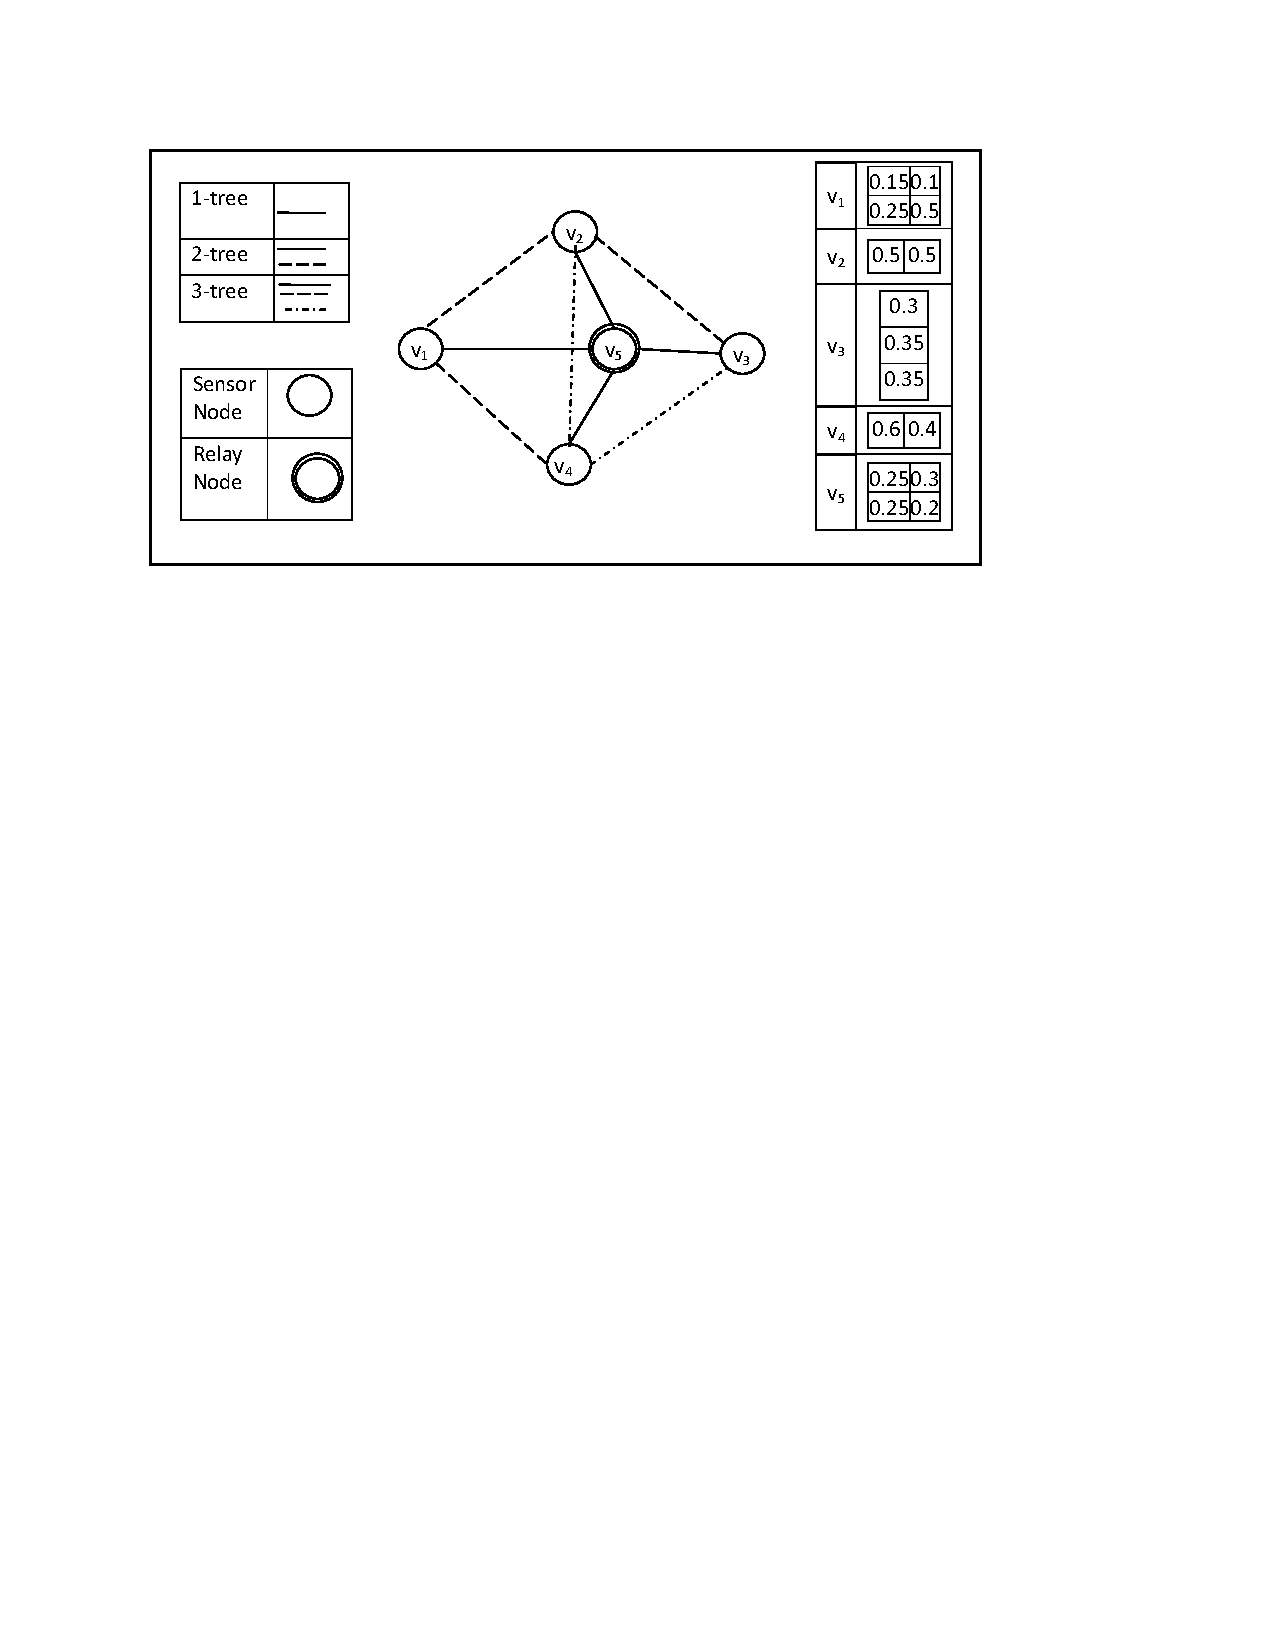
\includegraphics[width=6 in, height=2.5 in]{Relay.pdf}
 \caption{A partial \(2\)-tree with \(6\) nodes.
}
\end{figure}
\begin{exmp}
\normalfont
Fig \ref{fig:relay1} illustrates a network of 6 nodes where $v_1,v_2,v_3$ and $v_4$ are target nodes and $v_5, v_6$ are relays. $v_5$ is enhancing the connectivity of the network but $v_6$ is not  increasing the connectivity. So we can simply ignore $v_6$ and measure the connectivity from $v_1$ to $v_5$
\end{exmp}
\subsection{Problem Statement}
In this section we define the problem.
\begin{defi}[The $Conn(G,Tar)$ Problem]
\normalfont
We are given, $V$ the set of all nodes where each node $v\in V$ is located in a set of regions, $R_v=\{r_{(v,1)},r_{(v,2)},....\}$  with probability $p(r_{(v,i})$ where $i=1,2,...$.
$Rel\in V$ is the set of relay nodes and $Tar\in V$ is the set of target nodes where $V=Rel\cup Tar$. Also, if $x\in V$ and $y\in V$ are two nodes where $x$ can be located into one of it's locality set and $y$ can be located into one of it's locality set that they can communicate with each other then there is a link between $x$ and $y$, denoted by $(x,y)\in E$. Here we use relay nodes to enhance the performance of the network but we are interested to find out the probability $Conn(G,Tar)$ that all target nodes $Tar$ are connected.
\end{defi}
\subsection{Key Data Structures}
We already know from section \ref{subsec:kds} that a typical row in a table is key-value mapping. A key consists of 
i). partitions ii). regional set iii). target node attach. We explain them this section.


\begin{itemize}
\item[i)] partitions: There can be more than one partition associated with each row. Each partition consists with one or more node. We use braces to distinguish each partition. Two or more nodes are in the same partition means they can communicate each other when they are in regions indicated by regional set. For example in the key $\{v_1,v_2\}^{(1,1)}_{(1)}{v_3}^{(2)}_{(0)}$, there are two partitions including $\{v_1,v_2\}$ and $\{v_3\}$. Also node $v_1$ can reach node $2$ when they are both in region $1$ of their corresponding locality set but neither node $v_1$ nor node $v_2$  from region 1 can reach node 3 when node $v_3$ is in region 2 of it's locality set.
\item[ii).] regional set: The regional set of a partition consists of the position of corresponding node in the locality set. The regional set is indicated as a superscript of partition and is surrounded by parentheses. For example in the key $\{v_1,v_2\}^{(1,1)}_{(1)}{v_3}^{(2)}_{(0)}$, there are two regional sets $(1,1)$ and $(2)$ associated with two partitions $\{v_1,v_2\}$ and $\{v_3\}$ respectively. More specifically the partition-regional set pair $\{v_1,v_2\}^{(1,1)}$ indicates that node $v_1$ and $v_2$ are both located in region $1$ of their corresponding locality set.
\item[iii).] Target node attach: The target node attach associates with every partition. If there is one or more target node in a partition then the value of target node attach is 1 otherwise it is 0. In the above example we indicate the target node attach as a subscript of the partition. First partition in the above key $v_1$ and $v_2$ are target nodes so as a subscript we put 1 and for second partition we simply put 0 to indicate that $v_3$ is a relay node.
\end{itemize}

\begin{table}[!htb]
    %\caption{Global caption}
    \begin{minipage}{.3\linewidth}
      %\caption{$T_1(v_1,v_2,v_3)$}
      \centering
     \begin{tabular}{cc}
\multicolumn{2}{c}{$T_1(v_1,v_2,v_3)$}                           \\ \hline
\multicolumn{1}{|c}{.} & \multicolumn{1}{|c|}{.} \\ \hline
\multicolumn{1}{|l}{$\{v_1,v_2\}^{(1,1)}_{(1)} \{v_3\}^{(2)}_{(0)}$} & \multicolumn{1}{|l|}{$0.002$} \\ \hline
                             \multicolumn{1}{|c}{.} & \multicolumn{1}{|c|}{.} \\ \hline               
                   \multicolumn{1}{|c}{.} & \multicolumn{1}{|c|}{.} \\ \hline
                   \multicolumn{1}{|c}{.} & \multicolumn{1}{|c|}{.} \\ \hline        
\end{tabular}
    \end{minipage}%
    \begin{minipage}{.05\linewidth}
        \begin{tabular}{c}
     $ \times$\\
        \end{tabular}
    \end{minipage}%
     \begin{minipage}{.3\linewidth}
      %\caption{$T_1(v_1,v_2,v_3)$}
      \centering
     \begin{tabular}{cc}
\multicolumn{2}{c}{$T_2(v_1,v_3,v_4)$}                           \\ \hline
\multicolumn{1}{|c}{.} & \multicolumn{1}{|c|}{.} \\ \hline
\multicolumn{1}{|l}{$\{v_1\}^{(1)}_{(1)}\{v_3,v_4\}^{(2,1)}_{(1)}$} & \multicolumn{1}{|l|}{$0.008$} \\ \hline
                   \multicolumn{1}{|c}{.} & \multicolumn{1}{|c|}{.} \\ \hline               
                   \multicolumn{1}{|c}{.} & \multicolumn{1}{|c|}{.} \\ \hline
                   \multicolumn{1}{|c}{.} & \multicolumn{1}{|c|}{.} \\ \hline        
\end{tabular}
    \end{minipage}%
      \begin{minipage}{.06\linewidth}
        \begin{tabular}{c}
     $ \Rightarrow$\\
        \end{tabular}
    \end{minipage}%
     \begin{minipage}{.3\linewidth}
      %\caption{$T_1(v_1,v_2,v_3)$}
      \centering
     \begin{tabular}{cc}
\multicolumn{2}{c}{$Temp(v_1,v_2,v_3,v_4)$}                           \\ \hline
\multicolumn{1}{|c}{.} & \multicolumn{1}{|c|}{.} \\ \hline
  \multicolumn{1}{|l}{$\{v_1,v_2\}^{(1,1)}_{(1)}\{v_3,v_4\}^{\{2,1\}}_{(1)}$} & \multicolumn{1}{|l|}{$0.0008$} \\ \hline         
                   \multicolumn{1}{|c}{.} & \multicolumn{1}{|c|}{.} \\ \hline                 
                   \multicolumn{1}{|c}{.} & \multicolumn{1}{|c|}{.} \\ \hline
                   \multicolumn{1}{|c}{.} & \multicolumn{1}{|c|}{.} \\ \hline        
\end{tabular}
    \end{minipage}\\
    \begin{minipage}{1.0\linewidth}
       \centering
  
        \begin{tabular}{c}
Figure 3 a). Merging two table into $Temp$
        \end{tabular}
    \end{minipage}\\
     \begin{minipage}{.4\linewidth}
      %\caption{$T_1(v_1,v_2,v_3)$}
      \centering
     \begin{tabular}{cc}
\multicolumn{2}{c}{$Temp(v_1,v_2,v_3,v_4)$}                           \\ \hline
\multicolumn{1}{|c}{.} & \multicolumn{1}{|c|}{.} \\ \hline
  \multicolumn{1}{|l}{$\{v_1,v_2\}^{(1,1)}_{(1)}\{v_3,v_4\}^{(2,1)}_{(1)}$} & \multicolumn{1}{|l|}{$0.0008$} \\ \hline         
                   \multicolumn{1}{|c}{.} & \multicolumn{1}{|c|}{.} \\ \hline                 
                   \multicolumn{1}{|c}{.} & \multicolumn{1}{|c|}{.} \\ \hline
                   \multicolumn{1}{|c}{.} & \multicolumn{1}{|c|}{.} \\ \hline        
\end{tabular}
    \end{minipage}%
     \begin{minipage}{.06\linewidth}
   
        \begin{tabular}{c}
     $ \Rightarrow$\\
        \end{tabular}
    \end{minipage}%
    \begin{minipage}{.3\linewidth}
      %\caption{$T_1(v_1,v_2,v_3)$}
      \centering
     \begin{tabular}{cc}
\multicolumn{2}{c}{$Temp(v_2,v_3,v_4)$}                           \\ \hline
\multicolumn{1}{|c}{.} & \multicolumn{1}{|c|}{.} \\ \hline
  \multicolumn{1}{|l}{$\{v_2\}^{(1)}_{(1)}\{v_3,v_4\}^{(2,1)}_{(1)}$} & \multicolumn{1}{|l|}{$0.0008$} \\ \hline         
                   \multicolumn{1}{|c}{.} & \multicolumn{1}{|c|}{.} \\ \hline                 
                   \multicolumn{1}{|c}{.} & \multicolumn{1}{|c|}{.} \\ \hline
                   \multicolumn{1}{|c}{.} & \multicolumn{1}{|c|}{.} \\ \hline        
\end{tabular}
    \end{minipage}\\
      \begin{minipage}{1.0\linewidth}
       \centering
            \begin{tabular}{c}
Figure 3 b). Deleting node $v_1$ from $Temp$
        \end{tabular}
    \end{minipage}\\
\end{table}

\subsection{Main function}

\begin{itemize}
\item Step 8: check whether or not the node $v_i$, we are going to eliminate is a relay node. If $v_i$ is relay node, It goes to next step otherwise it goes to step $10$.
\item Step 9: search every partition in every row of the table $Temp$ for node $v_i$. It deletes node $v_i$ from every partition that contains node $v_i$. It also updates the regional sets of corresponding partitions from which $v_i$ was deleted by removing the corresponding regions of $v_i$.
\item Step 10: If $v_i$ is sensor node then it goes to next step.
\item Step 11: search every partition in every row of table $Temp$ for $v_i$. If the partitions that contains $v_i$ consists of more than one node then remove $v_i$ from that partitions. It also removes the location information of $v_i$ from the regional sets corresponding to those partitions.
If a partition contains $v_i$ itself this kind of partition is called bad partition. The algorithm simply ignore bad partition.
\end{itemize}
\begin{algorithm} [H]
\Indm
\KwIn{ a UWSN $G=(V,E)$ is a partial $k$-tree where each node, $v\in V$  can be located into a set of regions $R_v=\{r_{(v,1)},r_{(v,2)}...\}$ with probability,    
  $\{p(r_{(v,1)}),p(r_{(v,2)})...\}$ and $(x,y)\in E$ if $x\in V$ can be located one of it's locality set and $y\in V$ can be located one of it's locality set, so that they reach each other. A set of target nodes $Tar=\{v_1,v_2,...\}$ where $Tar\subset V$. A set of relay nodes $Rel=\{v_1,v_2,...\}$ where $Rel\subset V$. $PES$ is a perfect elimination sequence $(v_1,v_2,...,v_{n-k})$ of $G$.}
\KwOut{ Prob, a solution to the input instance.}
\textbf {Notation:} $Temp$ is a map from keys to probabilities.\\
%\noline
\Indp
\nl \textbf{Initialize } every clique by  a table.\\
\nl\For{$i=1,2,...,n-k$}
{
 \nl node $v_i$ is associated with $k$-cliques, $K_{(v_i,1)},K_{(v_i,2)},..,K_{(v_i,k)}$ \\
 //$T_{(v_i,1)},T_{(v_i,2)},..,T_{(v_i,k)}$ are the tables associated with cliques $K_{(v_i,1)},K_{(v_i,2)},..,K_{(v_i,k)}$ respectively \\
\nl $ Temp=T_{(v_i,1)}$  \\
 \nl \For{$j=2,3..,k$}
 {
  \nl $Temp=merge(Temp,T_{(v_i,j)})$\\
 }
 // clique $K_{(v_i,base)}$ is the base clique and table $T_{(v_i,base)}$ is the base table of node $v_i$
  \nl $Temp=merge(Temp,T_{(v_i,base)})$\\
\nl \If{$v_i$ is a relay node}{
\nl remove node $v_i$ from $Temp$ and assign the result to $T_{(v_i,base)}$ after updating the regional set.
}
\nl \Else{
\nl Remove $v_i$ from all the partitions of $Temp$ except the partition with $v_i$ itself and assign the result to $T_{(v_i,base)}$ after updating the regional set.\\
//We simply ignore the row where there is a partition of $v_i$ itself.}
}

\nl \Return{Prob=$\sum$(All probability for single partition in the remaining table)}
\caption{Function Main$(G$, $\textbf{R}$, $Tar$, $Rel$, $p(r_{(v,i)})$, $PES )$}
\end{algorithm}
\subsection{Merge Function }
\begin{algorithm}[H]
\Indm  
\KwIn{ Two tables $T_1$ and $T_2$ that share at least one common vertex}
\KwOut{A  table $T$}

\textbf{Notation} $C$ is a set of vertices and $Obj$ is a row of table $T$ and $Prob\_C$ is a double variable\\
\Indp
\nl \textbf{set} $C=$ the set of common vertices between $T_1$ and $T_2$ , set $Prob\_C=1$\\
 \nl \If{$C\neq \emptyset$}{
 \nl \ForEach{row $r$ in $T_1$}
 {
 \nl \ForEach{row $s$ in $T_2$}
 {
  \nl  $Obj.par=$pMerge($r.par$,$s.par$)\\
   \nl \ForEach{vertex $v_i$ in $Obj.par$ where $i=1,2,..,k+1$}
    {
   \nl $Obj.locmap[v_i]=r.locmap[v_i]||s.locmap[v_i]$\\
    }
    \nl \ForEach{node $v$ in every partition $P$ in $Obj.par$}
    {
    \nl \ForEach{node $u$ in every partition $Q$ in $s.par$}
    {
    \nl \If{$v==u$}
    {
   \nl $Obj.tAttach[P]=max(Obj.tAttach[P],s.tAttach[Q])$
    }
    }
     \nl \ForEach{node $w$ in every partition $T$ in $r.par$}
    {
    \nl \If{$v==w$}
    {
    \nl $Obj.tAttach[P]=max(Obj.tAttach[P],r.tAttach[T])$
    }
    }
    }
   \nl \ForEach{vertex  $v\in C$}
    {
   \nl $Prob\_C=Prob\_C*s.loc[v]$
    }
\nl $ Obj<Obj.par:Obj.loc>=\frac{Prob[r]\times Prob[s]}{Prob\_C}$\\
\nl Insert $Obj$ in $T$ as a row.\\
}
  }
  }
\nl \Return {Table T}

 \caption{Function merge($T_1,T_2$)}
\end{algorithm}

\begin{itemize}
\item Step 8: selects every node $v$ of every partition $P$ in the newly created row $Obj$.
\item Step 9: iterates every node $u$ of every partition $Q$ in the row $s$.
\item Step 10: check whether $u$ and $v$ are the same same node or not. If they are same then it goes to next step otherwise it goes to step 9.
\item Step 11: updates the target attach entry of partition $P$ by taking the max between the target attach entry of partition $P$ and target attach entry of partition $Q$.
\item Step 12: iterates every node $w$ of every partition $T$ in the row $r$.
\item Step 13: check whether $w$ and $v$ are the same same node or not. If they are same then it goes to next step otherwise it goes to step 9.
\item Step 11: updates the target attach entry of partition $P$ by taking the max between the target attach entry of partition $P$ and target attach entry of partition $T$.
\end{itemize}
\subsection{Simulation Results}
\begin{table}
 \begin{minipage}{.5\linewidth}
      \caption{Accuracy with respect to $k$}
      \centering
     \begin{tabular}{|c|c|c|c|c|c|c|}
     \hline
     k & Network I & Network IR & Network II & NeworkIIR & NetworkIII & Network IIIR \\
     \hline
      1 & 30.23 & 86.96 & 5.23 &22.27  &15.99 & 28.44\\\hline
	  2 & 53.72 & 96.72 & 17.55 & 59.43& 80.23&89.3\\\hline
	  3 &60.20 & 97.60 & 20.96 & 60.5& 83.3&92.3\\\hline
\end{tabular}
    \end{minipage}\\
   % \caption{Running time(RT) and accuracy increases with respect to $k$}
\end{table}   
    \begin{figure}

\begin{minipage}{.9\linewidth}
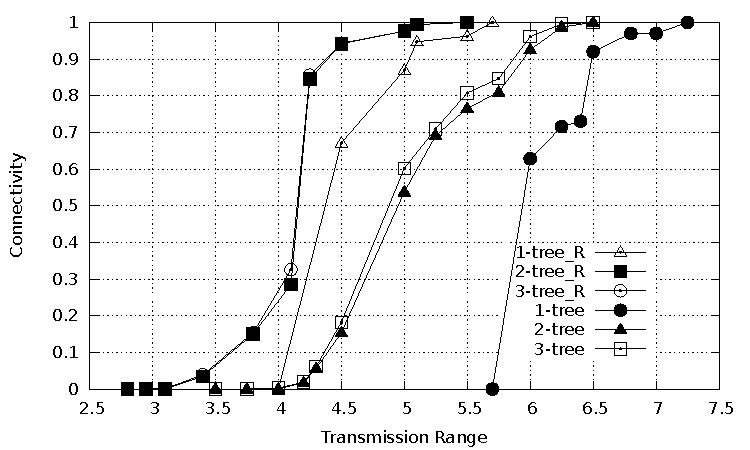
\includegraphics[width=6 in, height=2.6 in]{NetworkI_woR.pdf}
\caption{NetworkIII}
\end{minipage}

\end{figure}
% ------------------------------------------------------------
%\section{ References}
\bibliographystyle{plain} 
\bibliography{final}
% ------------------------------------------------------------
%\hLine{2 in}
\end{document}
